\chapter{Realization - Web Features}
\setcounter{minitocdepth}{1}
\minitoc
\newpage
\section{Introduction}
In this chapter, we will be discussing the two web-related sprints. We will provide a detailed explanation of the conception part, including a class diagram and a sequence diagram. Additionally, we will present the sprint backlog and include relevant screenshots of these sprints. Furthermore, we will showcase some code snippets to illustrate the implementation process.

\section{Sprint 1 - Recreating the Simple Template}

\subsection{Sprint Backlog}
In this section, we present the Sprint Backlog, detailing the tasks planned for developing shop visiting features. It is a concise list of user stories and specific actions that will guide us through the sprint.

\setlength{\LTleft}{0pt}
\begin{longtable}{|c|c|c|c|}
\hline
\textbf{Sprint} & \textbf{User Story} & \textbf{Task} & \textbf{ID} \\
\hline
1 & 1.1 & Implement the shop landing page & 1.0.1 \\
\hline
1 & 1.2 & Add functionality to load additional products & 1.0.2 \\
\hline
1 & 1.3 & Include social media links in the shop interface & 1.0.3 \\
\hline
1 & 1.4 & Implement a support team contact section & 1.0.4 \\
\hline
1 & 1.5 & Develop a search feature for specific products & 1.0.5 \\
\hline
1 & 1.6 & Create a checkout form for shop visitors & 1.0.6 \\
\hline
1 & 1.7 & Enable the ability to add items to the cart & 1.0.7 \\
\hline
1 & 1.8 & Implement the purchase functionality & 1.0.8 \\
\hline
1 & 1.9 & Add the option for shop visitors to accept or decline offers & 1.0.9 \\
\hline
\caption{Sprint 1 - Recreating the Simple Template}
\label{tab:sprint1_backlog}
\end{longtable}

\subsection{Design \& Implementation}
In this section, we will explore the design and implementation of the shop visiting process. We will begin by examining the backend design and implementation, followed by an analysis of the frontend design.

\subsubsection{Database Schema}
The database schema for the shop visiting process is shown in Figure \ref{fig:db_schema_sprint1}. It consists of the following tables:

\begin{figure}[H]
    \centering
    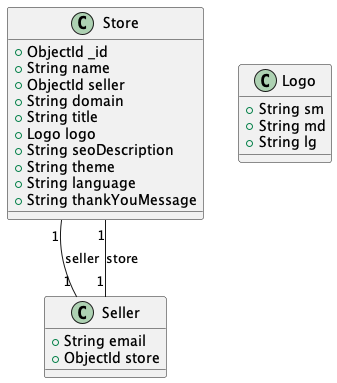
\includegraphics[width=0.5\textwidth]{images/sprintOneClass.png}
    \caption{Database Schema for Sprint 1}
    \label{fig:db_schema_sprint1}
\end{figure}


The class diagram illustrates the relationships between three main classes: \texttt{Store}, \texttt{Seller}, and \texttt{Logo}.

\begin{itemize}
    \item \textbf{Store Class:} Represents a shop with attributes such as an ID (\texttt{\_id}), name, associated seller, domain, title, logo, SEO description, theme, language, and a thank-you message. The \texttt{Logo} is a composite object with different sizes (small, medium, large).
    
    \item \textbf{Seller Class:} Represents the seller associated with a store, containing attributes like email and a reference to the \texttt{Store}.
    
    \item \textbf{Logo Class:} Contains attributes for the different sizes of logos (\texttt{sm}, \texttt{md}, \texttt{lg}).
    
    \item \textbf{Relationships:}
    \begin{itemize}
        \item Each \texttt{Store} is associated with a \texttt{Seller} through a one-to-one relationship.
        \item Conversely, each \texttt{Seller} is linked back to a \texttt{Store}, maintaining the one-to-one relationship.
    \end{itemize}
\end{itemize}

\subsubsection{Sequence Diagram}

The sequence diagram in Figure \ref{fig:sequence_diagram_sprint1} illustrates the interactions between the different components of the shop visiting process. The sequence of events is as follows:

\begin{figure}[H]
    \centering
    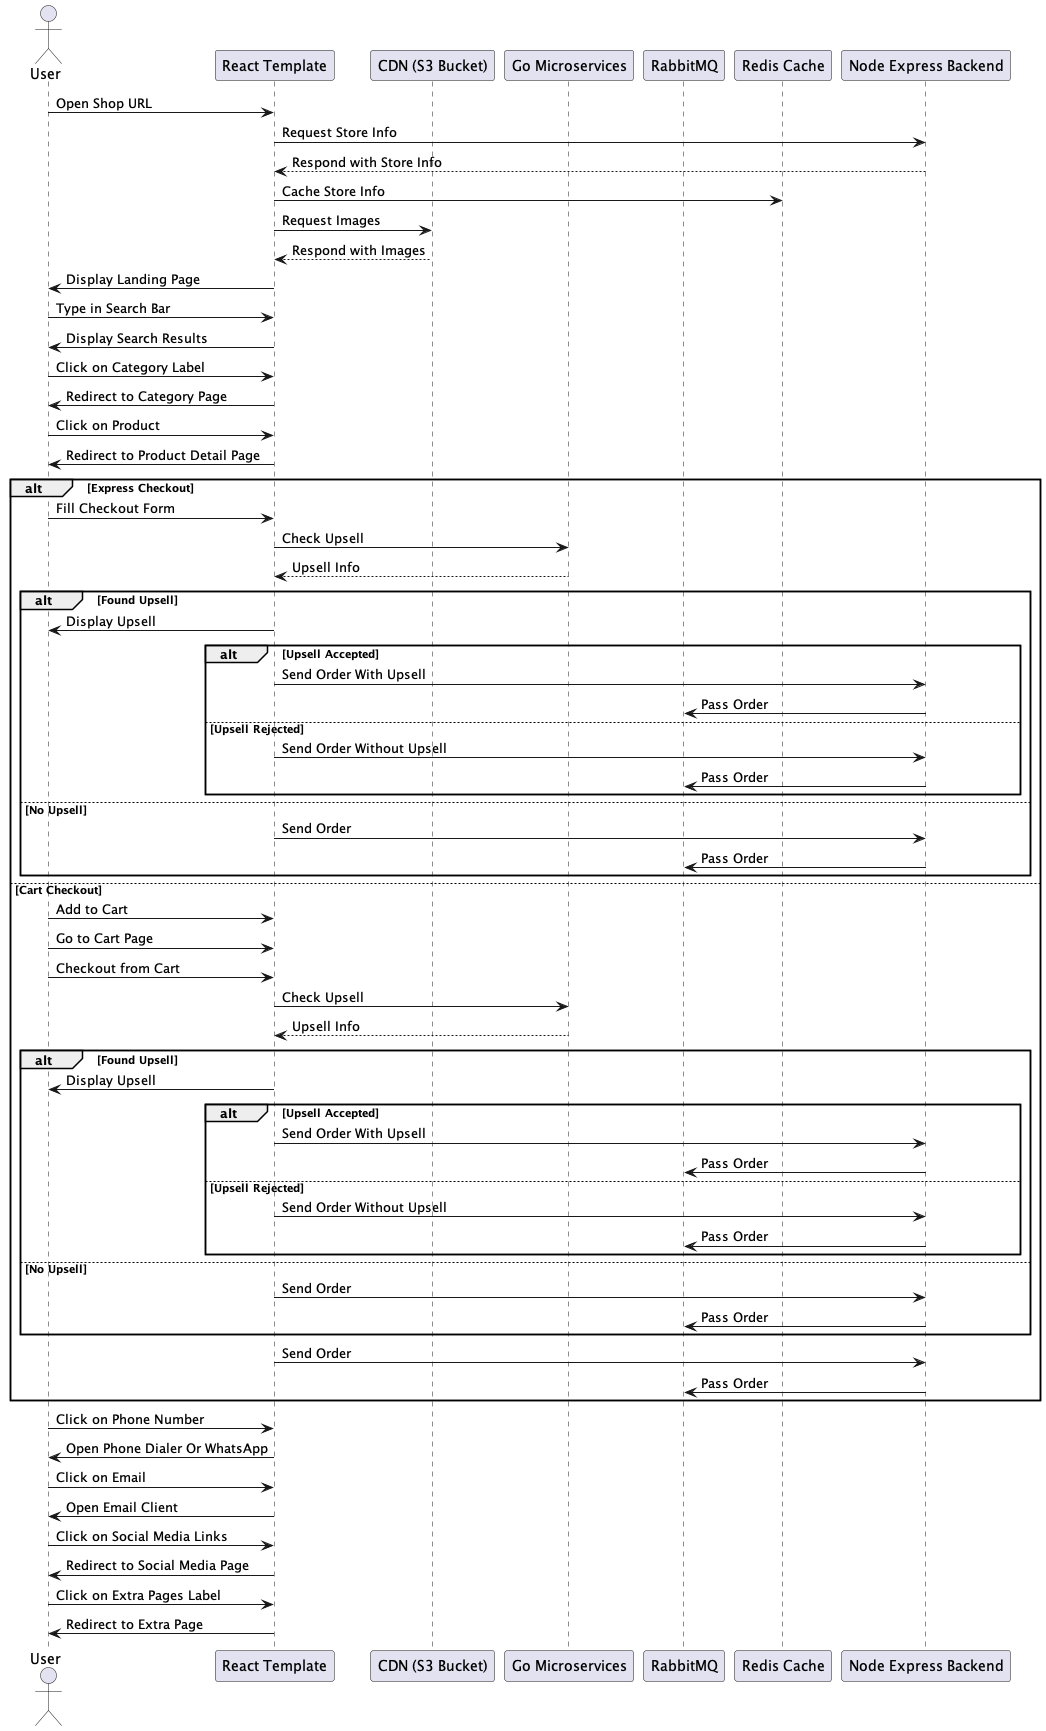
\includegraphics[width=0.8\textwidth]{images/sprintOneSequence.png}
    \caption{Sequence Diagram for Sprint 1}
    \label{fig:sequence_diagram_sprint1}
\end{figure}

\subsubsection{User Journey}

The user journey for the shop visiting process is as follows:

\begin{figure}[H]
    \centering
    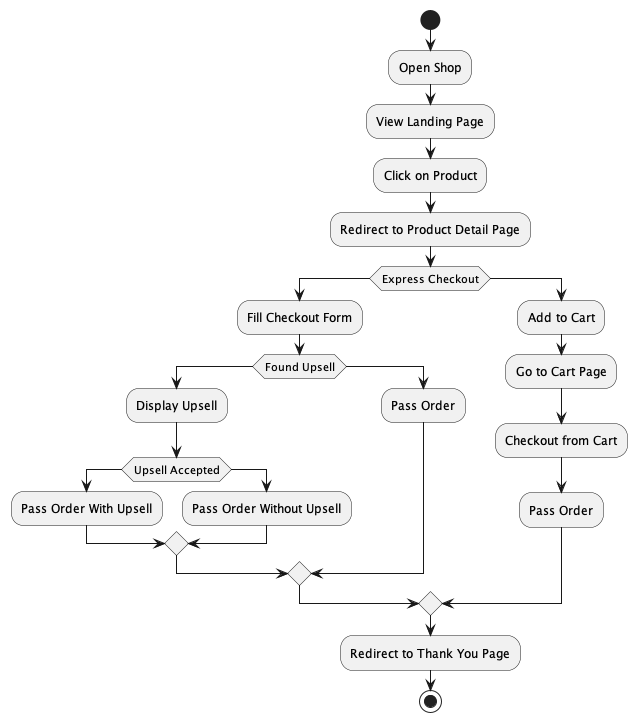
\includegraphics[width=0.8\textwidth]{images/sprintOneActivity.png}
    \caption{User Journey for Sprint 1}
    \label{fig:user_journey_sprint1}
\end{figure}

This activity diagram outlines the steps a shop visitor takes to buy a product:

\begin{itemize}
    \item The user opens the shop's website and views the landing page.
    \item The user clicks on a product, which redirects them to the product detail page.
    \item If the shop is configured for express checkout, the user fills out the checkout form. If an upsell is found, it is displayed to the user. The user can either accept or reject the upsell. Based on their choice, the order is passed with or without the upsell.
    \item If the shop is not configured for express checkout, the user adds the product to the cart, goes to the cart page, and proceeds to checkout from the cart. The order is then passed.
    \item Finally, the user is redirected to the thank you page, completing the purchase process.
\end{itemize}

\subsubsection{Screenshots - UI Design}

\begin{itemize}
    \item \textbf{Shop Landing Page:} The shop landing page is the first page a user sees when visiting a shop. It contains a list of products, a search bar, and social media links. Figures \ref{fig:shop_landing_page_one} and \ref{fig:shop_landing_page_two} shows the shop landing page.
    \begin{figure}[H]
        \centering
        \includegraphics[width=0.8\textwidth]{images/landingPage1.png}
        \caption{Shop Landing Page 1}
        \label{fig:shop_landing_page_one}
    \end{figure}
    \begin{figure}[H]
        \centering
        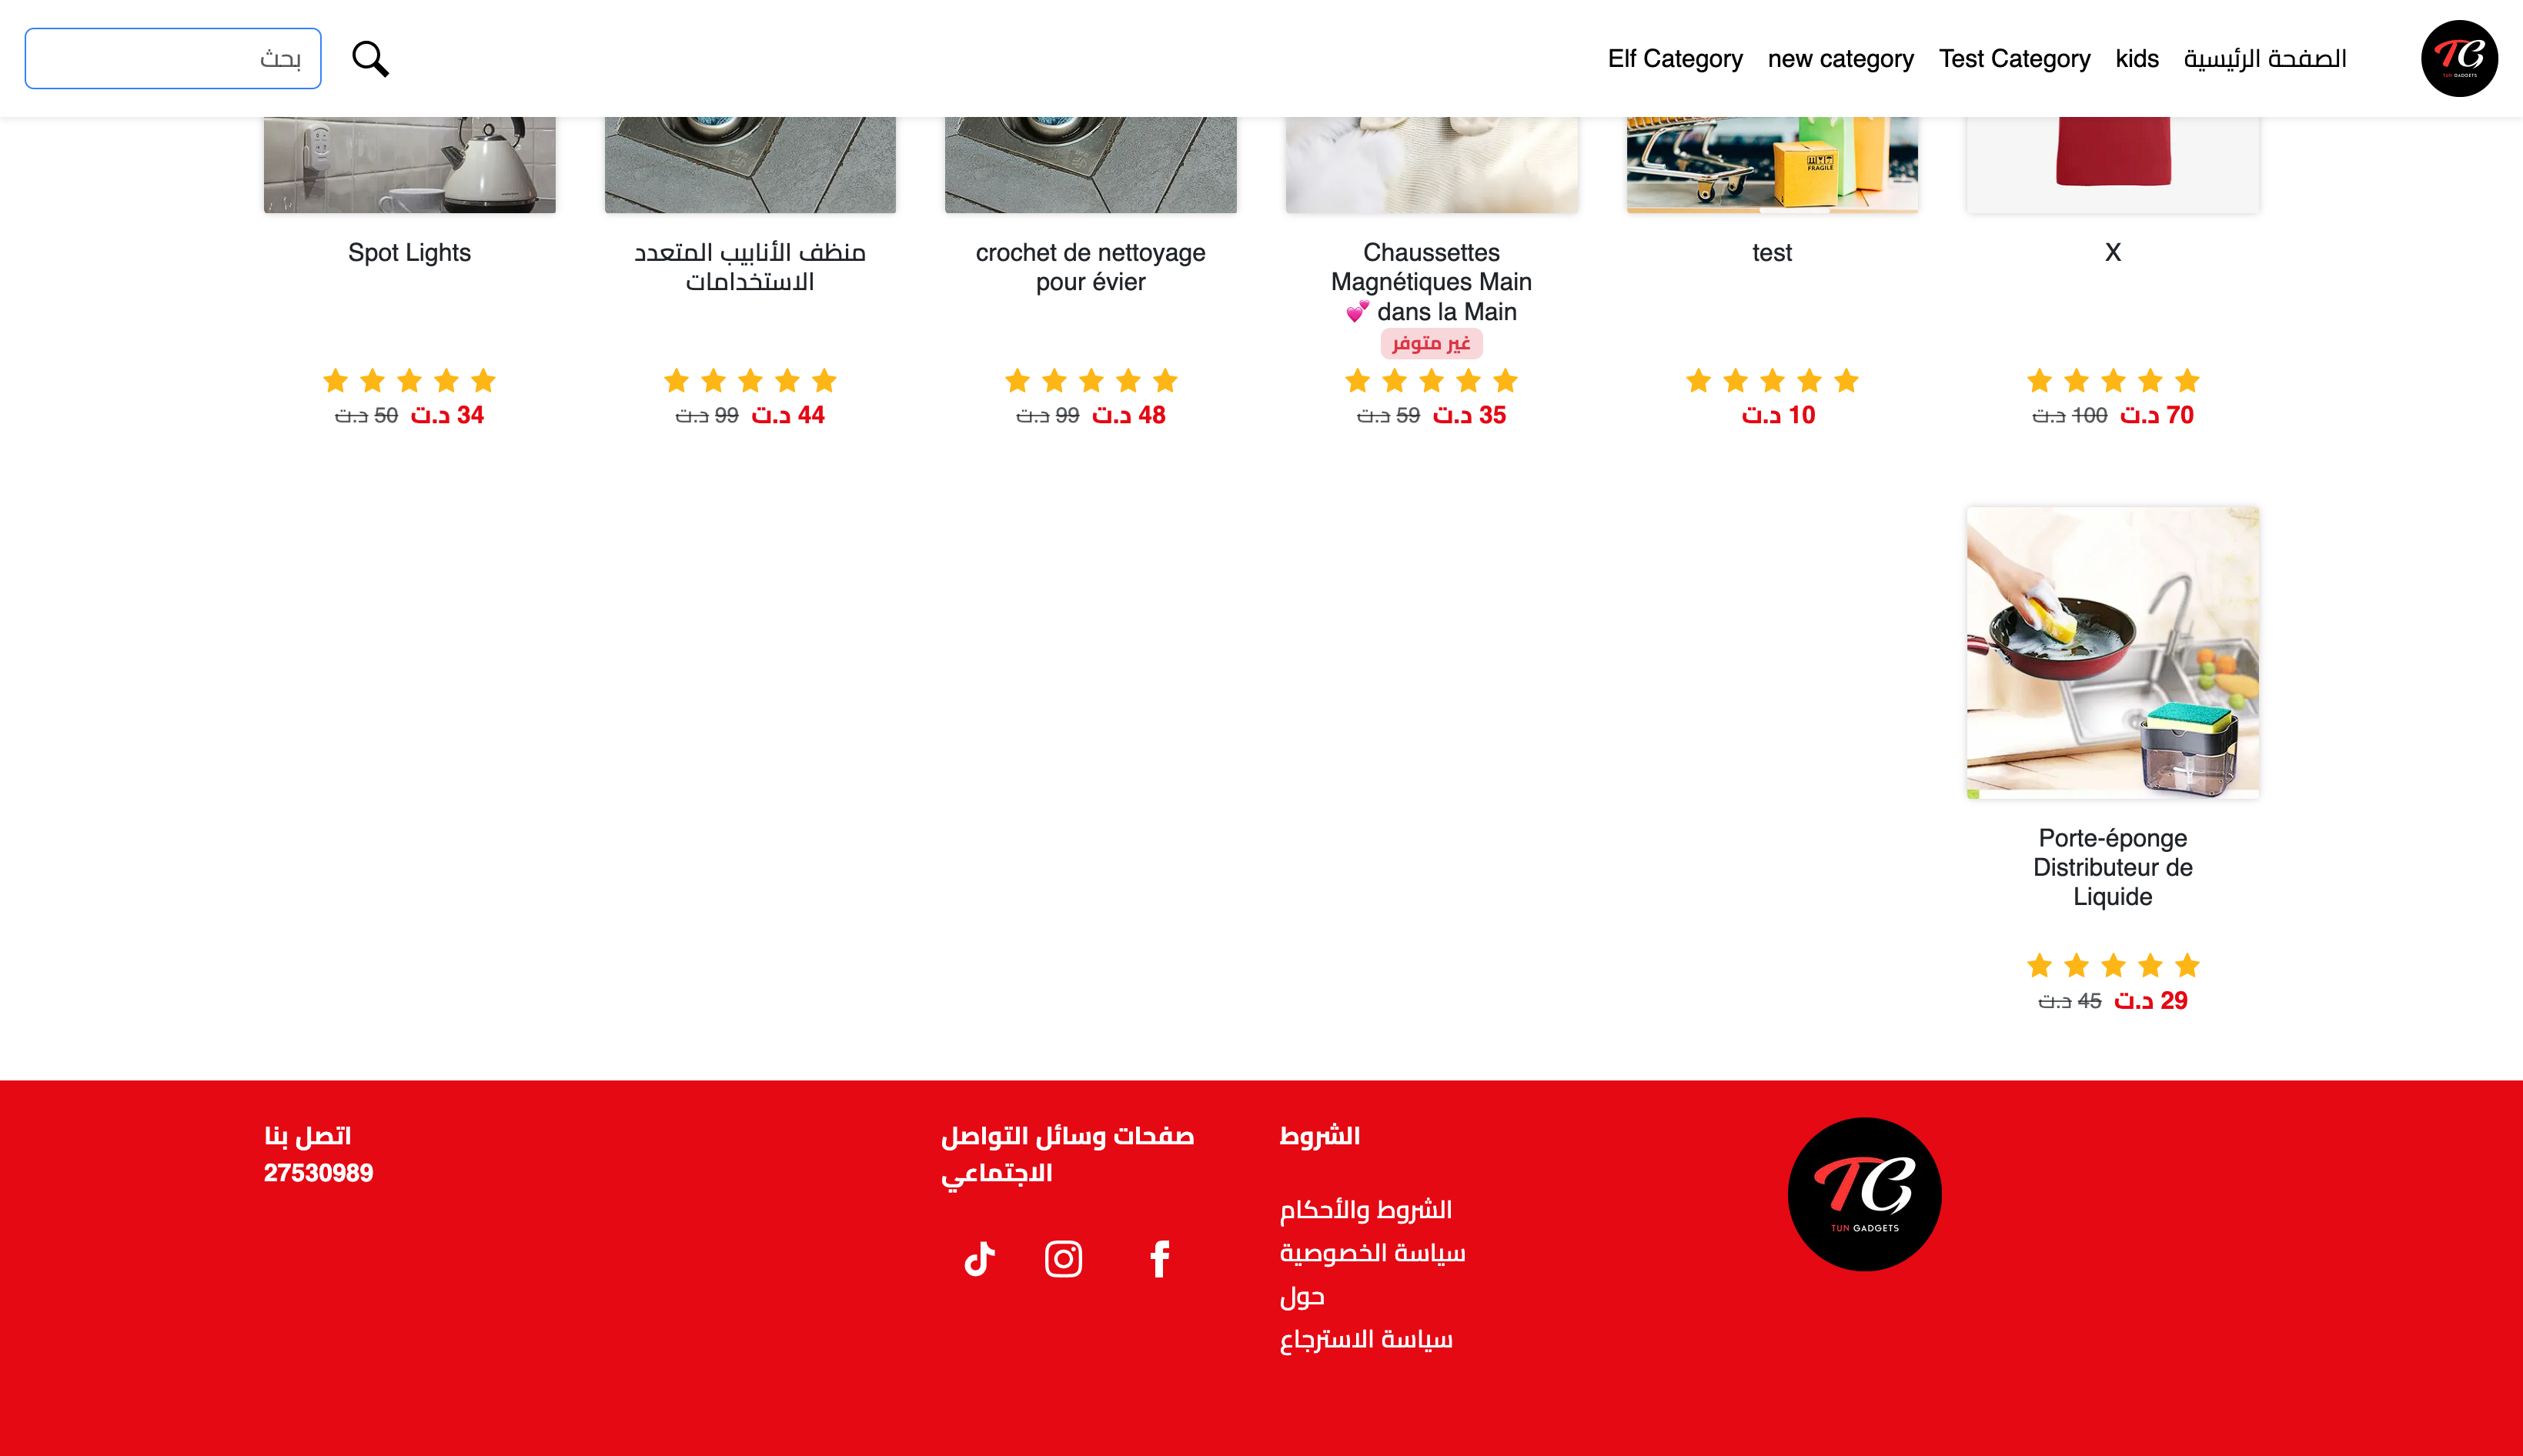
\includegraphics[width=0.8\textwidth]{images/landingPage2.png}
        \caption{Shop Landing Page 2}
        \label{fig:shop_landing_page_two}
    \end{figure}
    \item \textbf{Category Page:} The category page displays a list of products in a specific category. Figure \ref{fig:category_page} shows the category page.
    \begin{figure}[H]
        \centering
        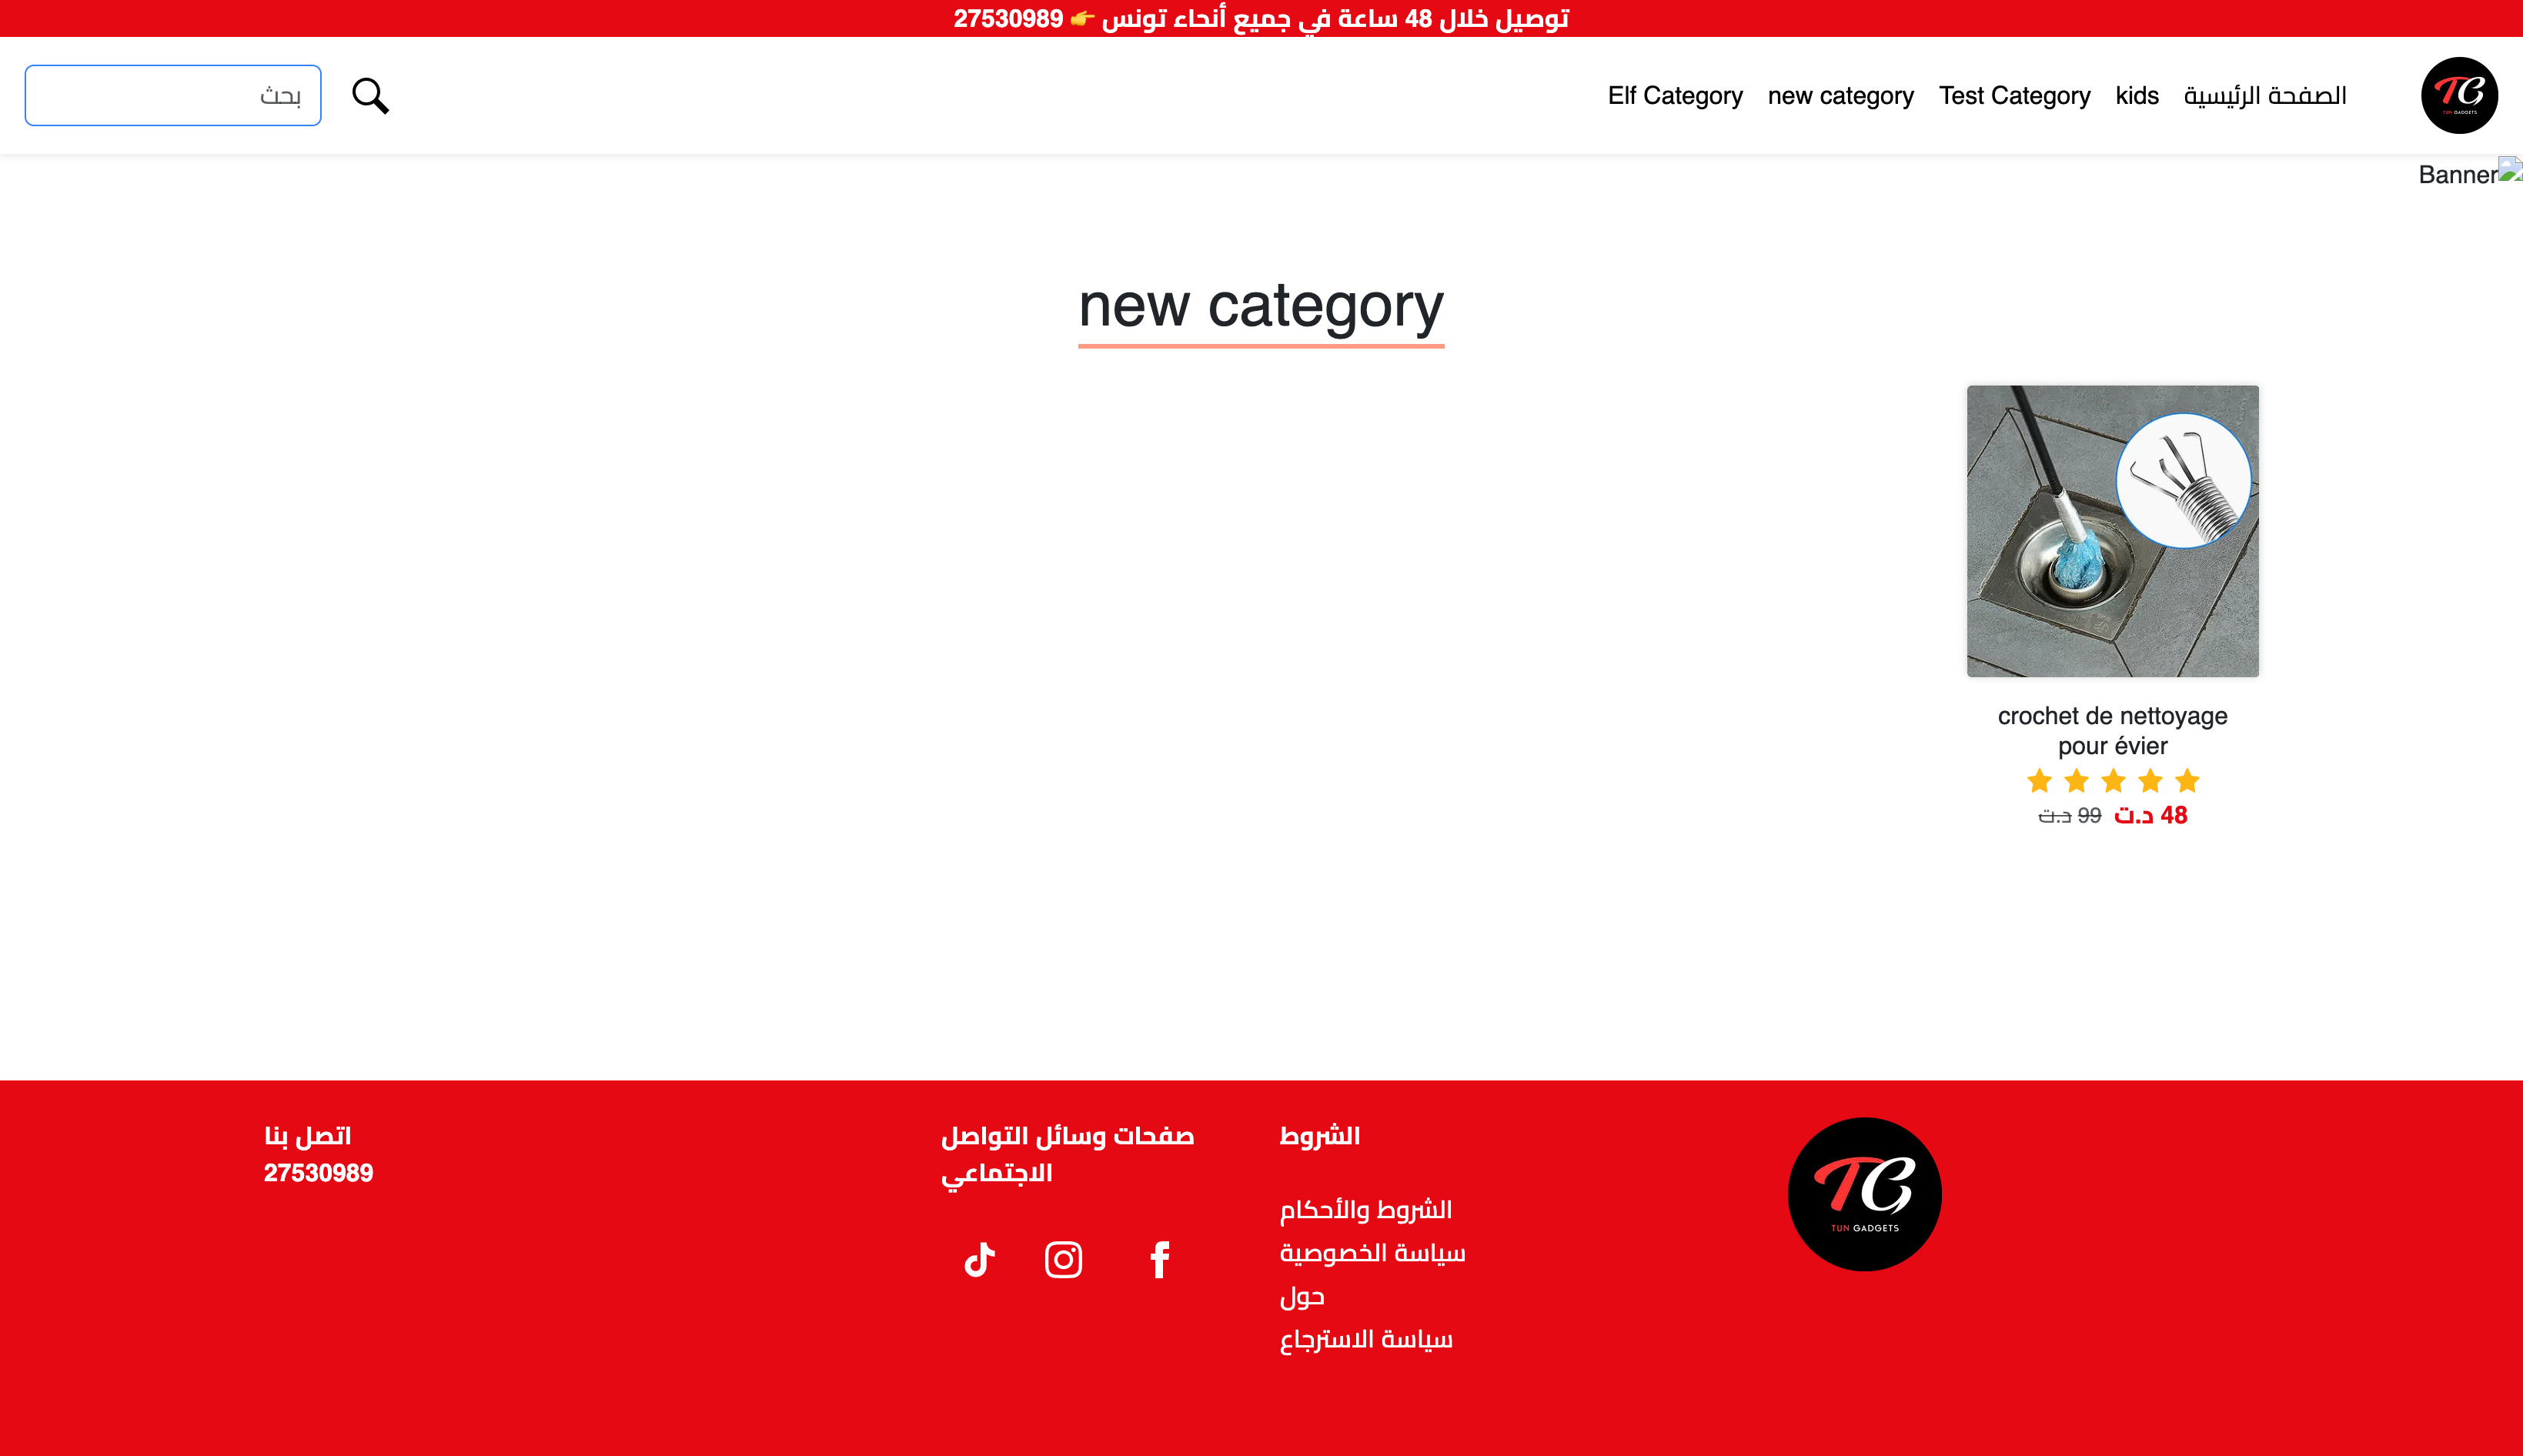
\includegraphics[width=0.8\textwidth]{images/categoryPage.png}
        \caption{Category Page}
        \label{fig:category_page}
    \end{figure}
    \item \textbf{Search Page:} The search page displays a list of products based on the user's search query. Figure \ref{fig:search_page} shows the search page.
    \begin{figure}[H]
        \centering
        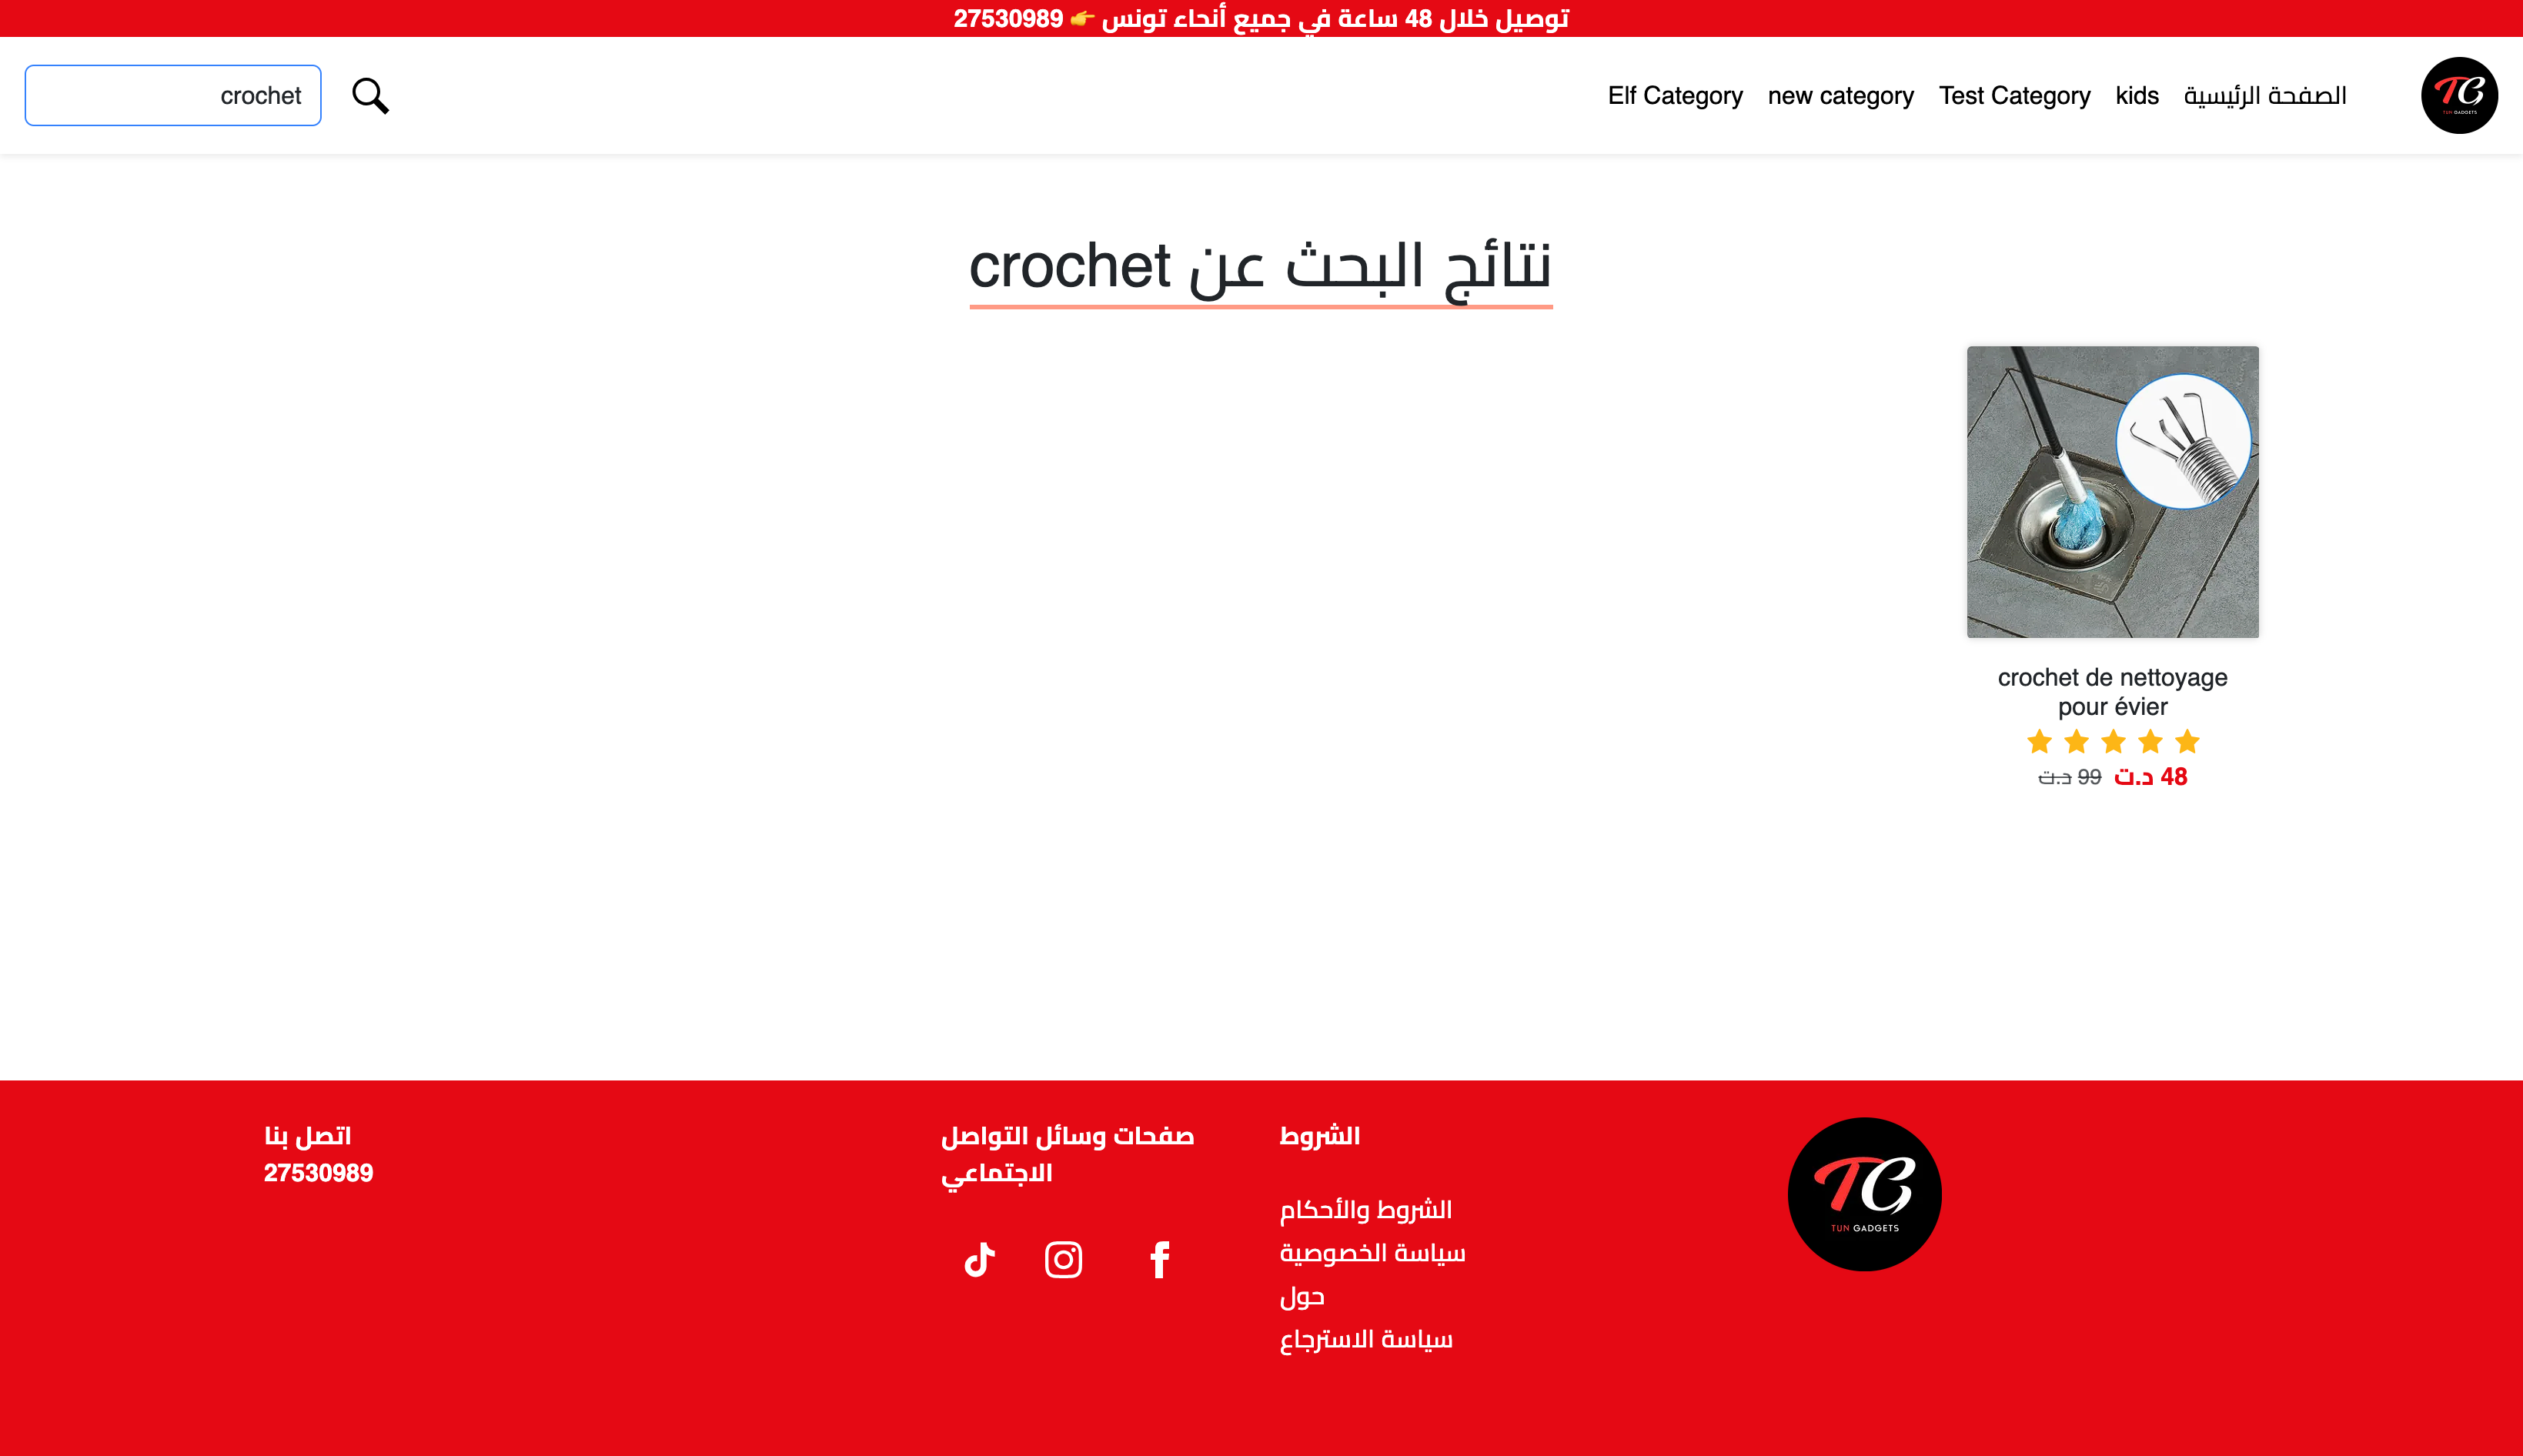
\includegraphics[width=0.8\textwidth]{images/searchPage.png}
        \caption{Search Page}
        \label{fig:search_page}
    \end{figure}
    \item \textbf{Extra Page (Ex: Refund \& Return Policy):} The extra page displays additional information about the shop, such as the refund and return policy. Figure \ref{fig:extra_page} shows the extra page.
    \begin{figure}[H]
        \centering
        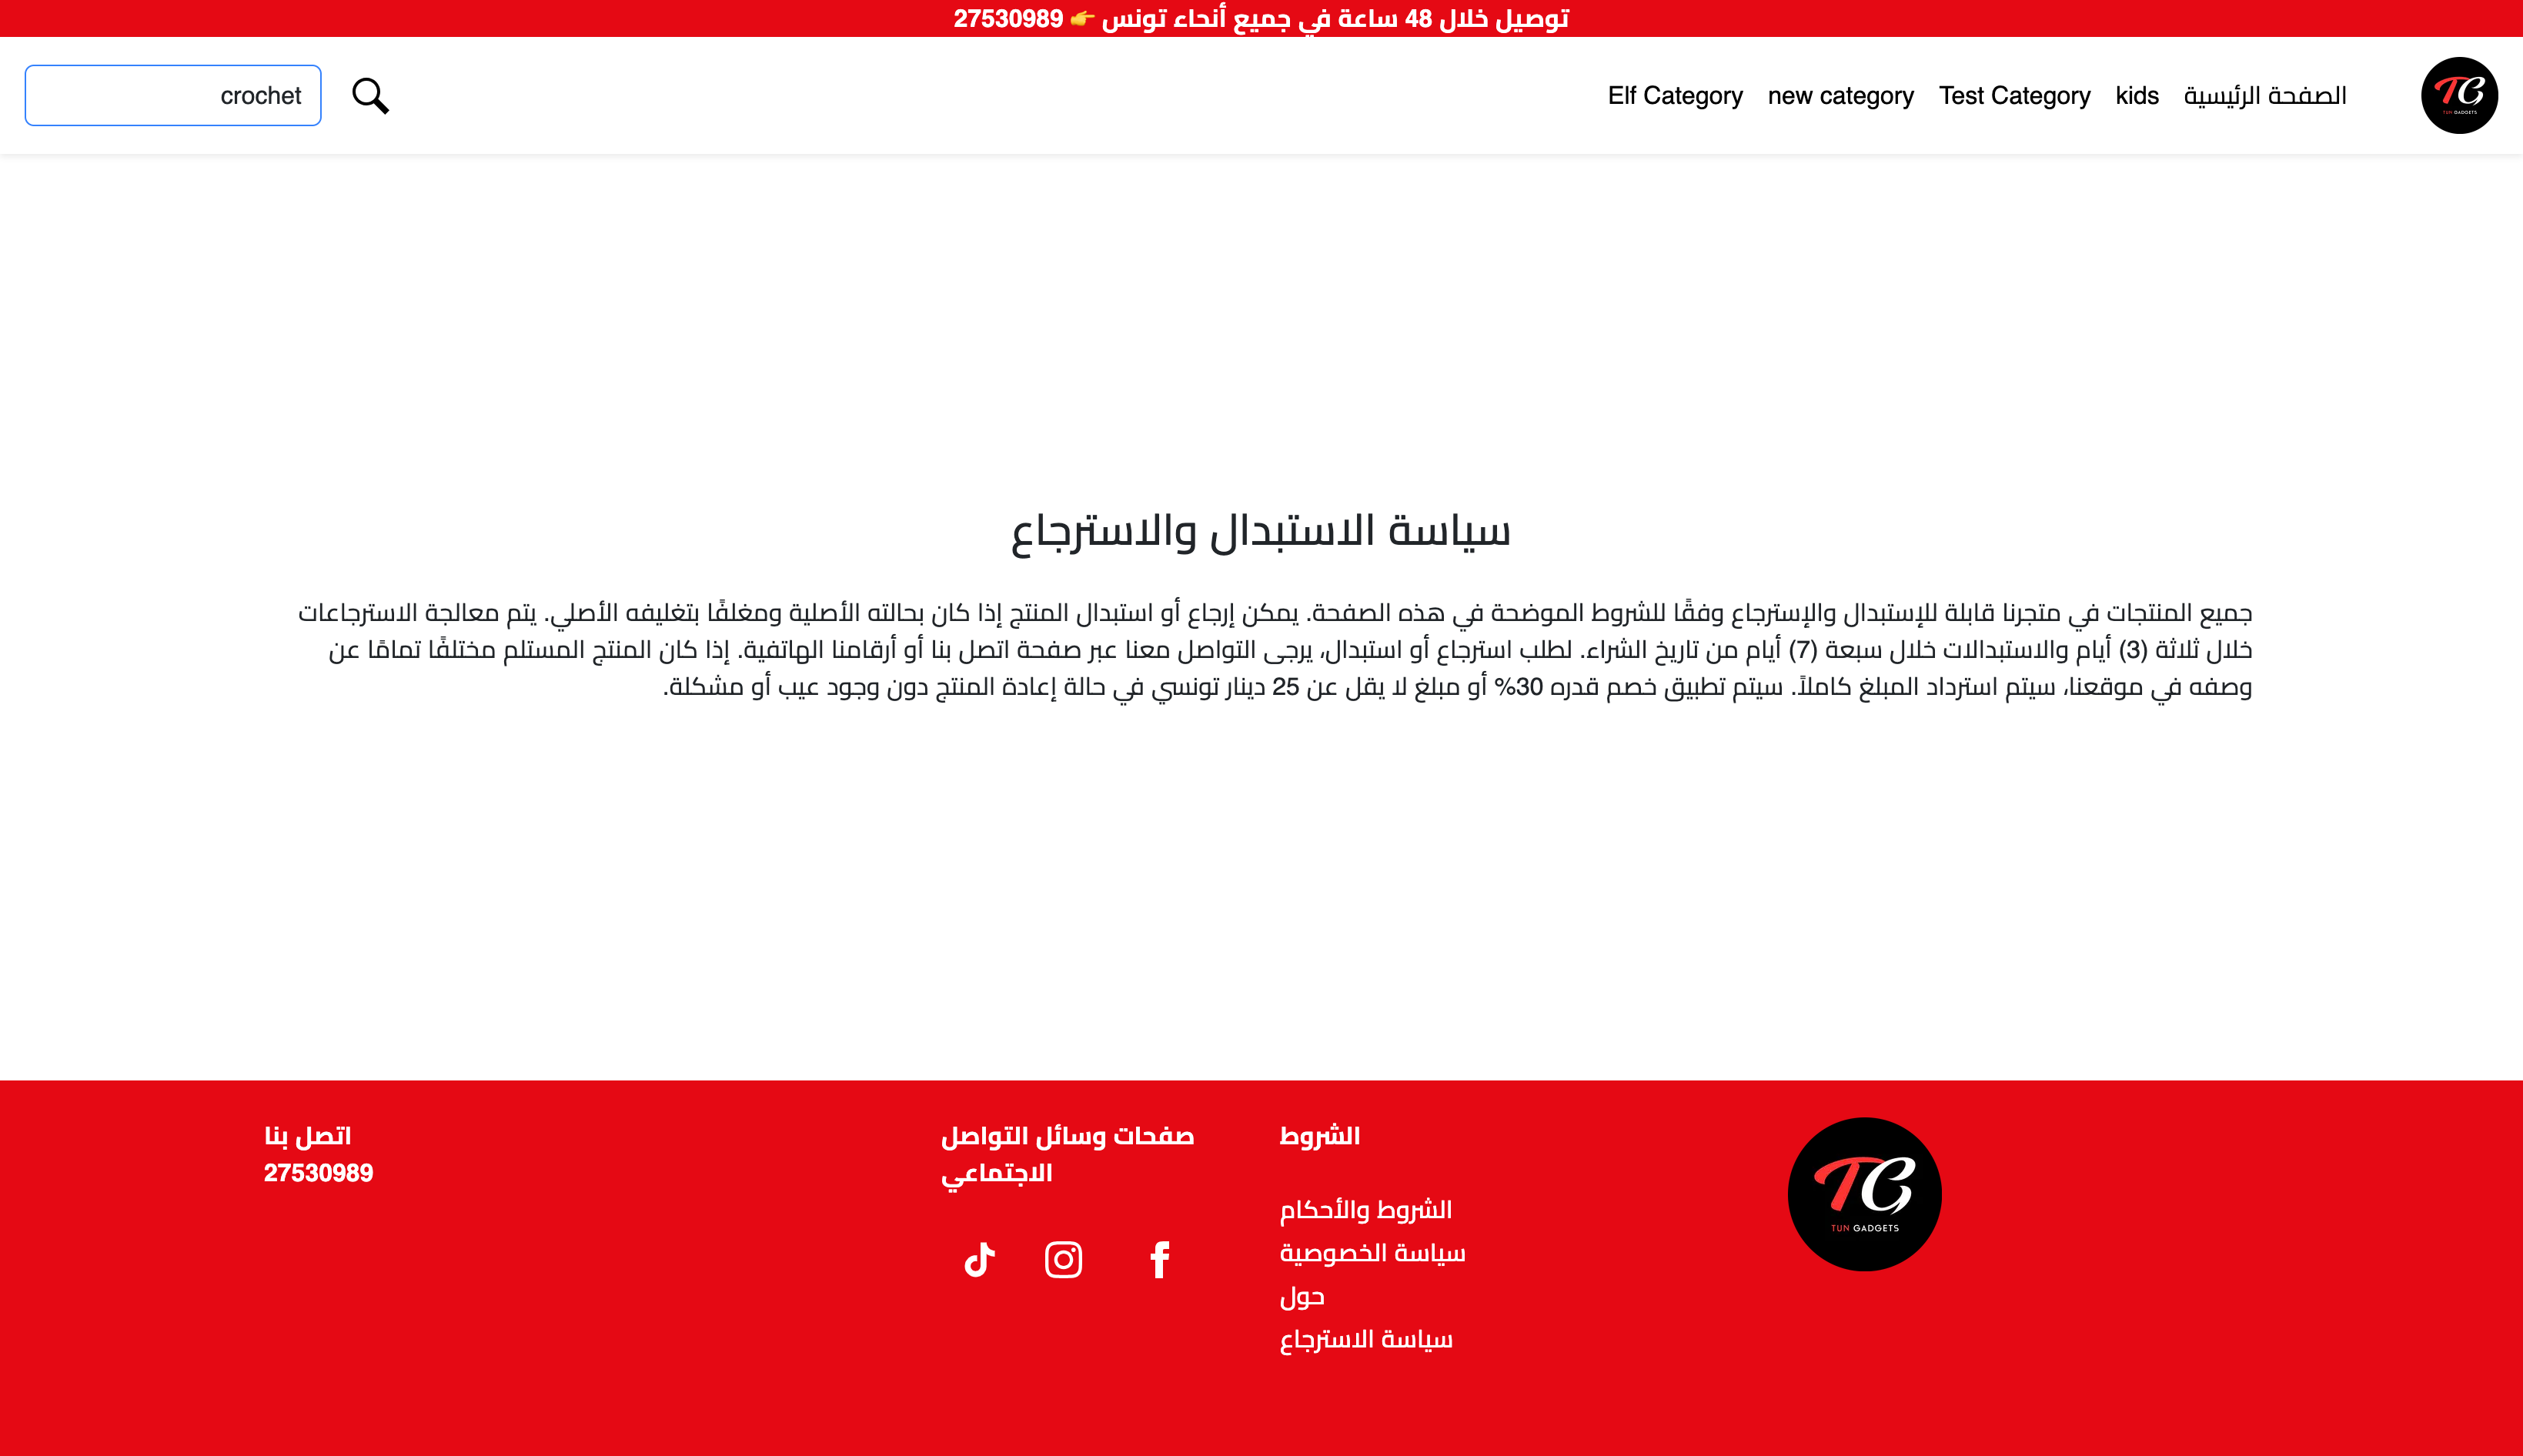
\includegraphics[width=0.8\textwidth]{images/extra_page.png}
        \caption{Extra Page}
        \label{fig:extra_page}
    \end{figure}
    \item \textbf{Product Detail Page:} The product detail page displays information about a specific product alonng with a checkout form and other clients opinions about it. Figures \ref{fig:product_detail_page_one}, \ref{fig:product_detail_page_two} and \ref{fig:product_detail_page_three} shows the product detail page.
    \begin{figure}[H]
        \centering
        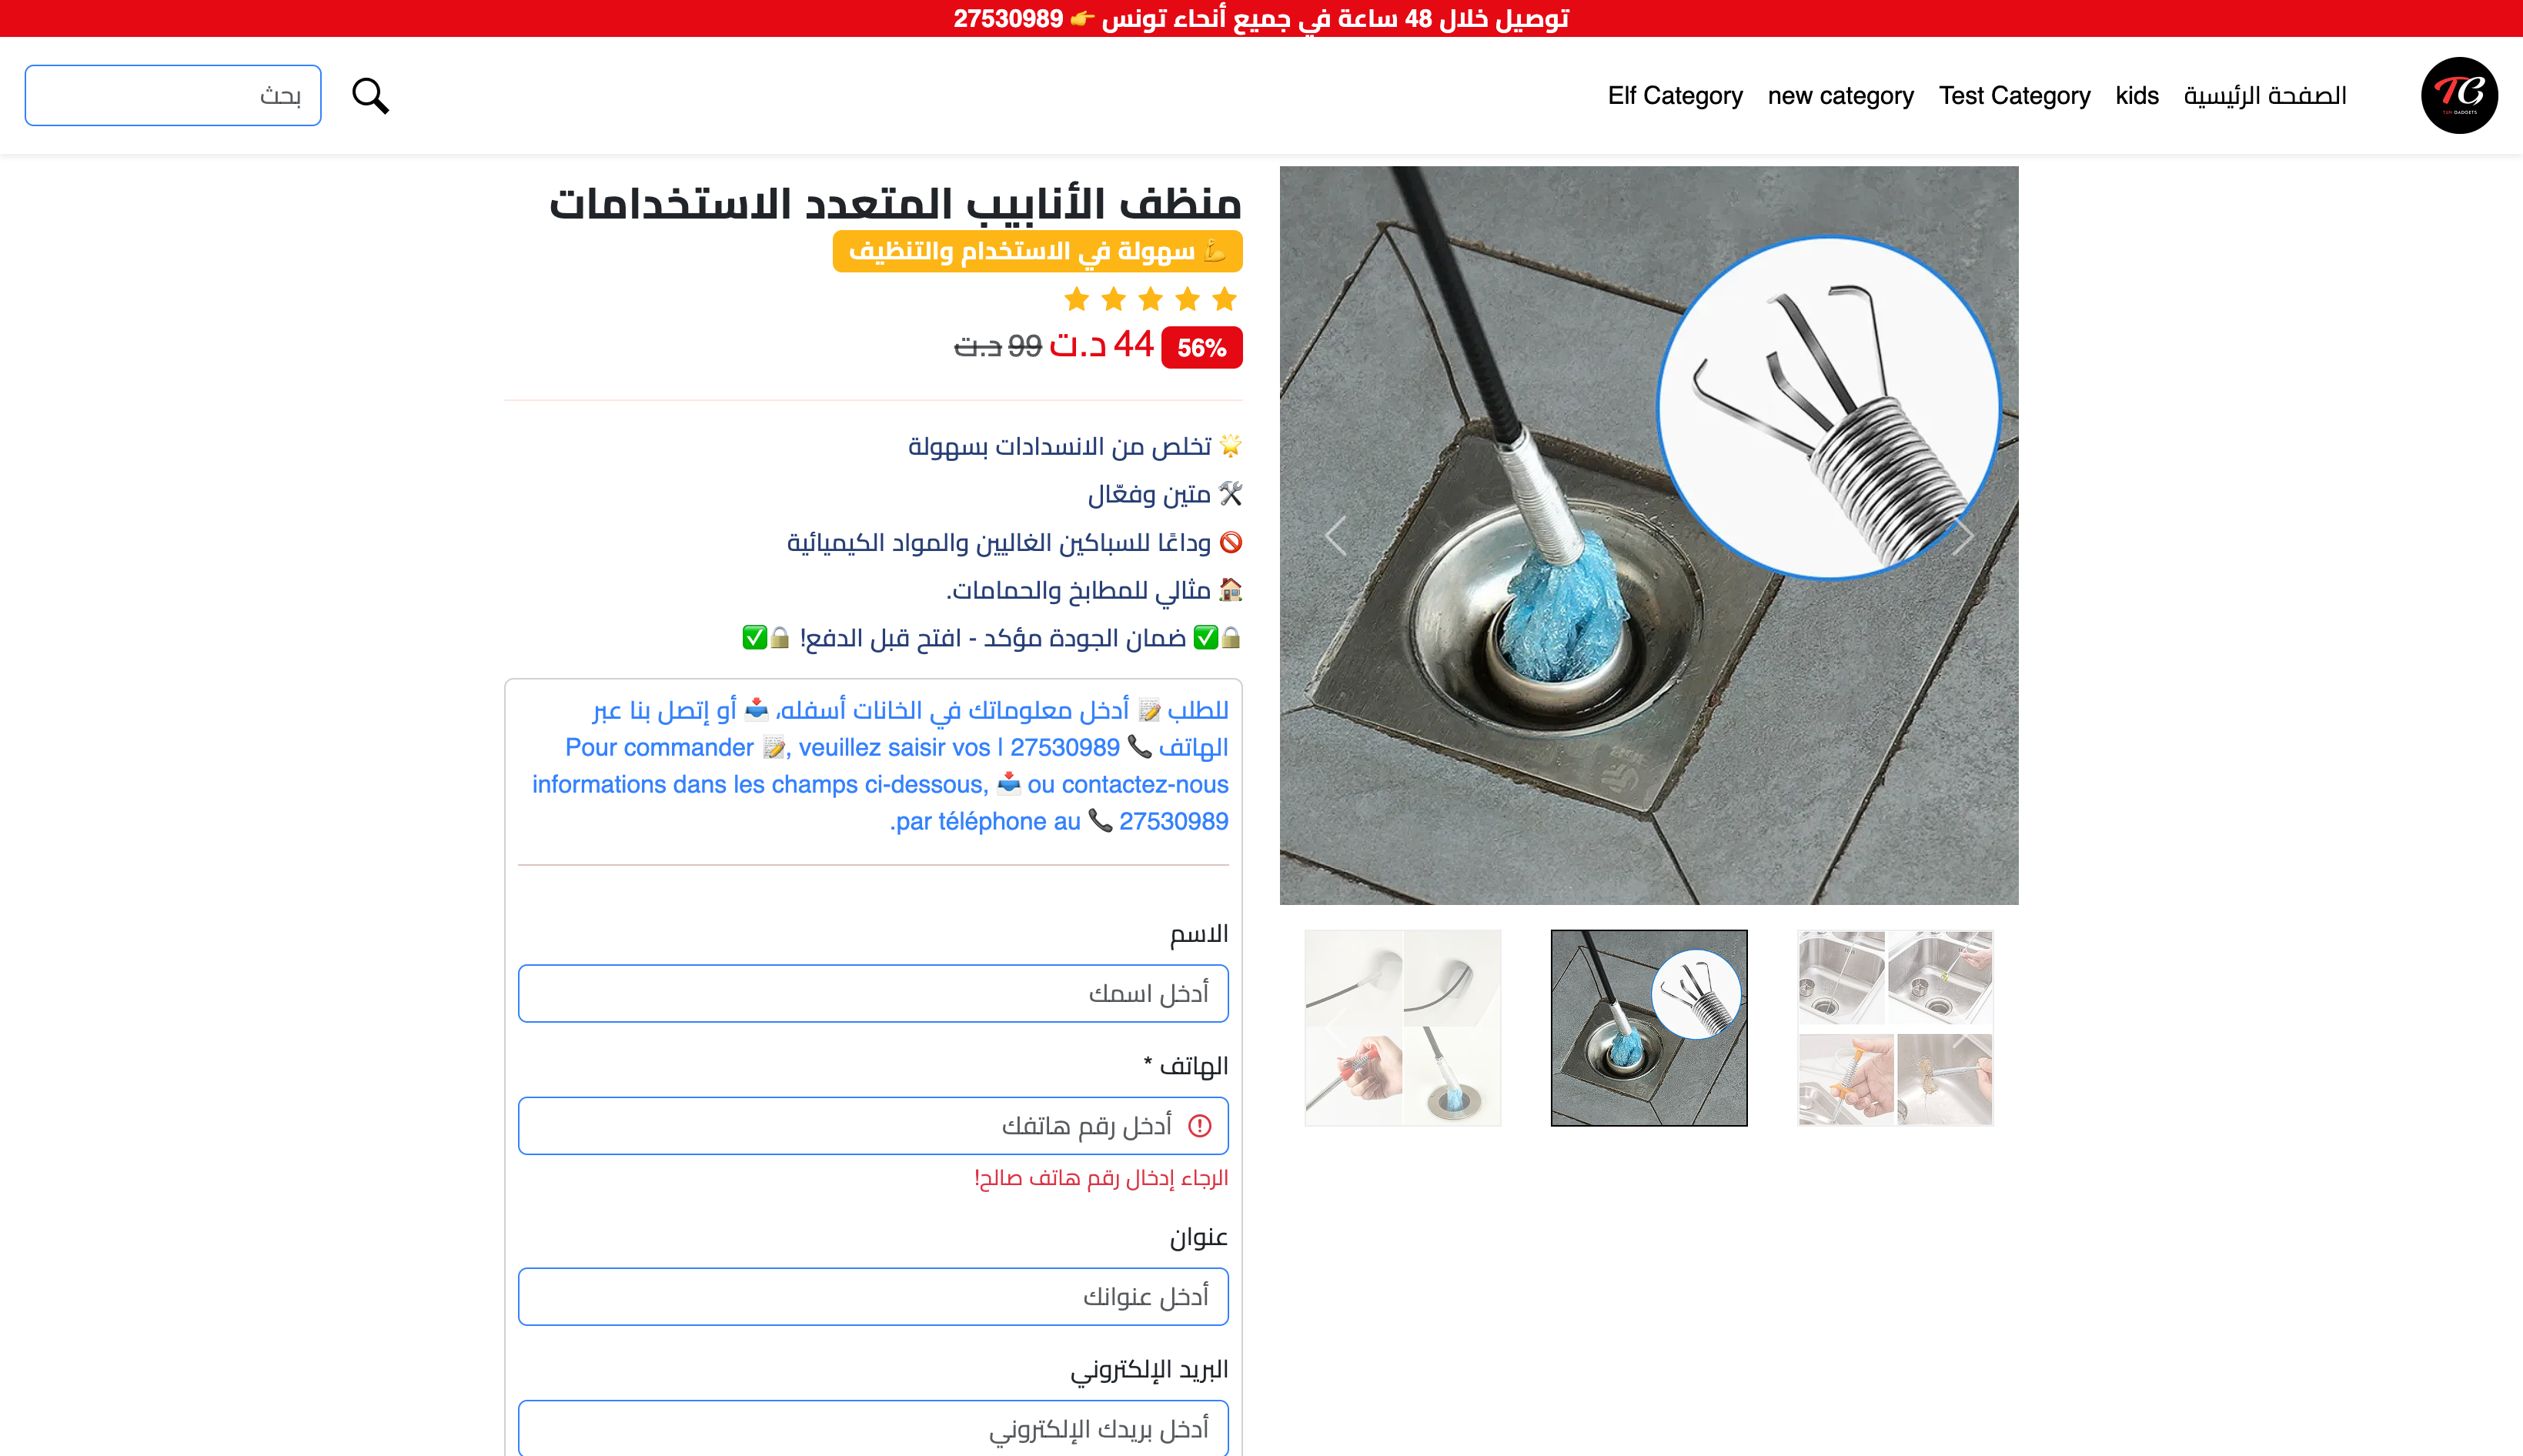
\includegraphics[width=0.8\textwidth]{images/productDetailPage1.png}
        \caption{Product Detail Page 1}
        \label{fig:product_detail_page_one}
    \end{figure}
    \begin{figure}[H]
        \centering
        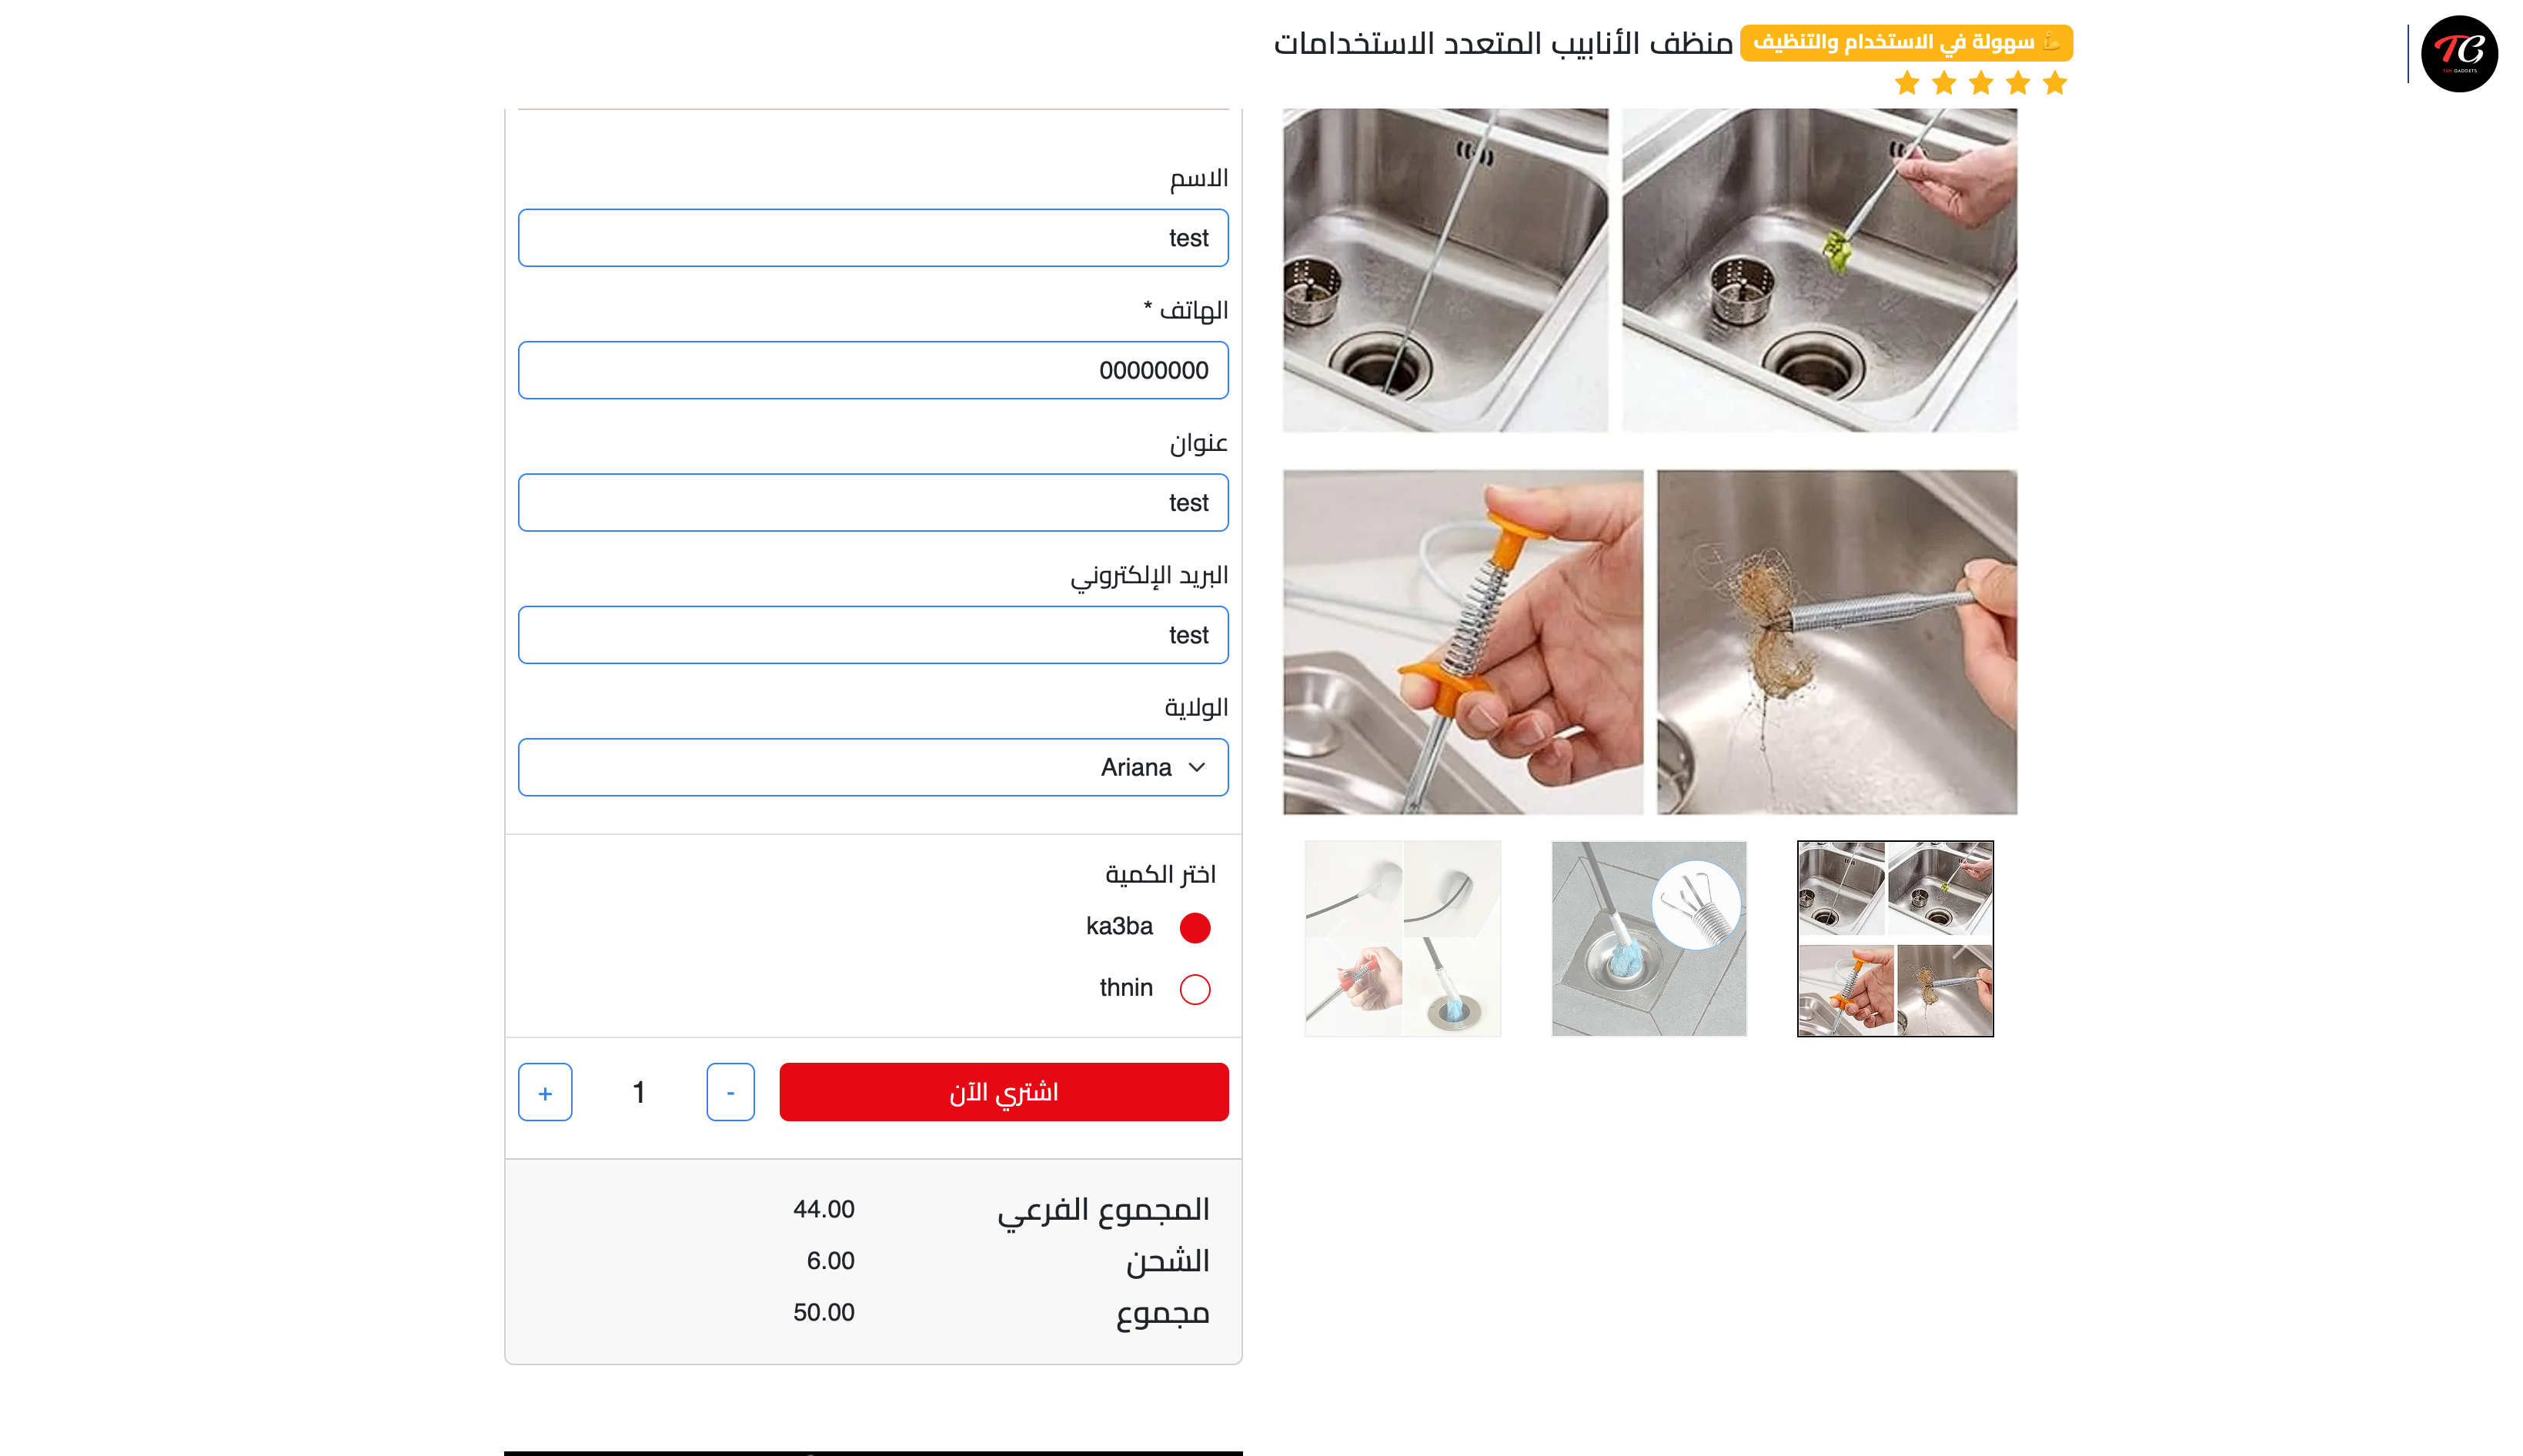
\includegraphics[width=0.8\textwidth]{images/productDetailPage2.png}
        \caption{Product Detail Page 2}
        \label{fig:product_detail_page_two}
    \end{figure}    
    \begin{figure}[H]
        \centering
        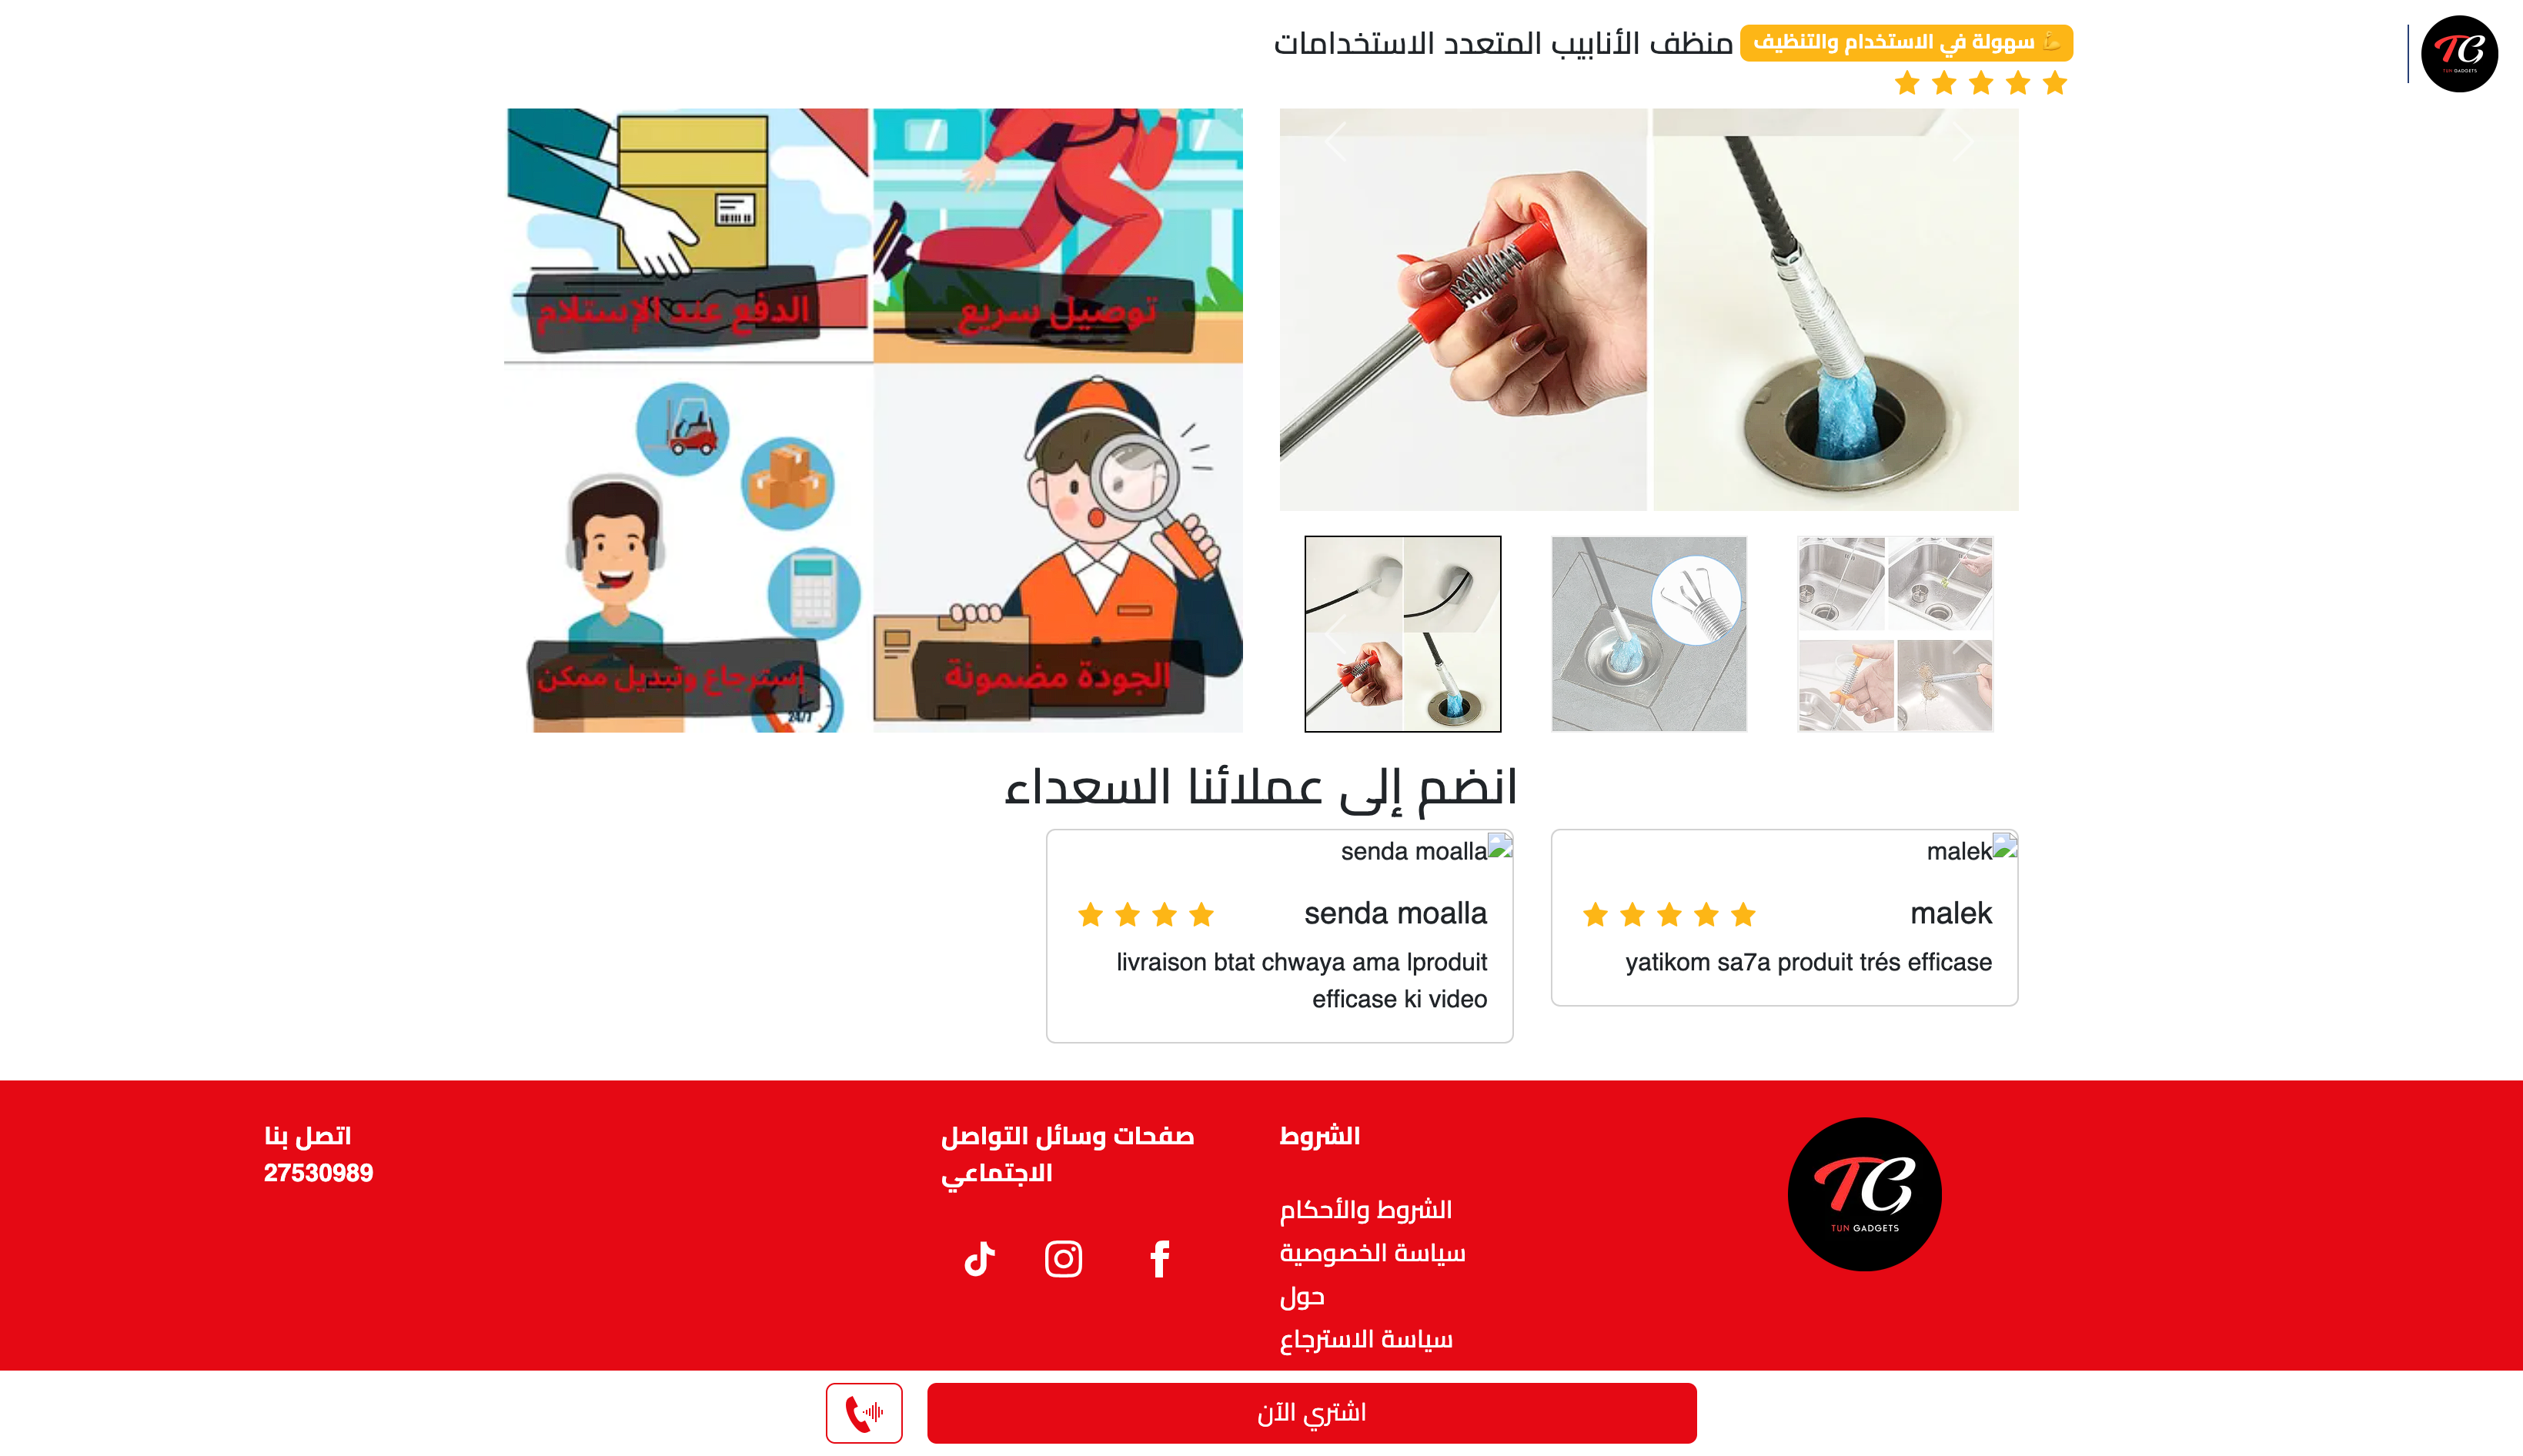
\includegraphics[width=0.8\textwidth]{images/productDetailPage3.png}
        \caption{Product Detail Page 3}
        \label{fig:product_detail_page_three}
    \end{figure}
    \item \textbf{Thank You Page:} The thank you page is displayed after a successful purchase. Figure \ref{fig:thank_you_page} shows the thank you page and figure \ref{fig:upsell} shows the upsell popup.
    \begin{figure}[H]
        \centering
        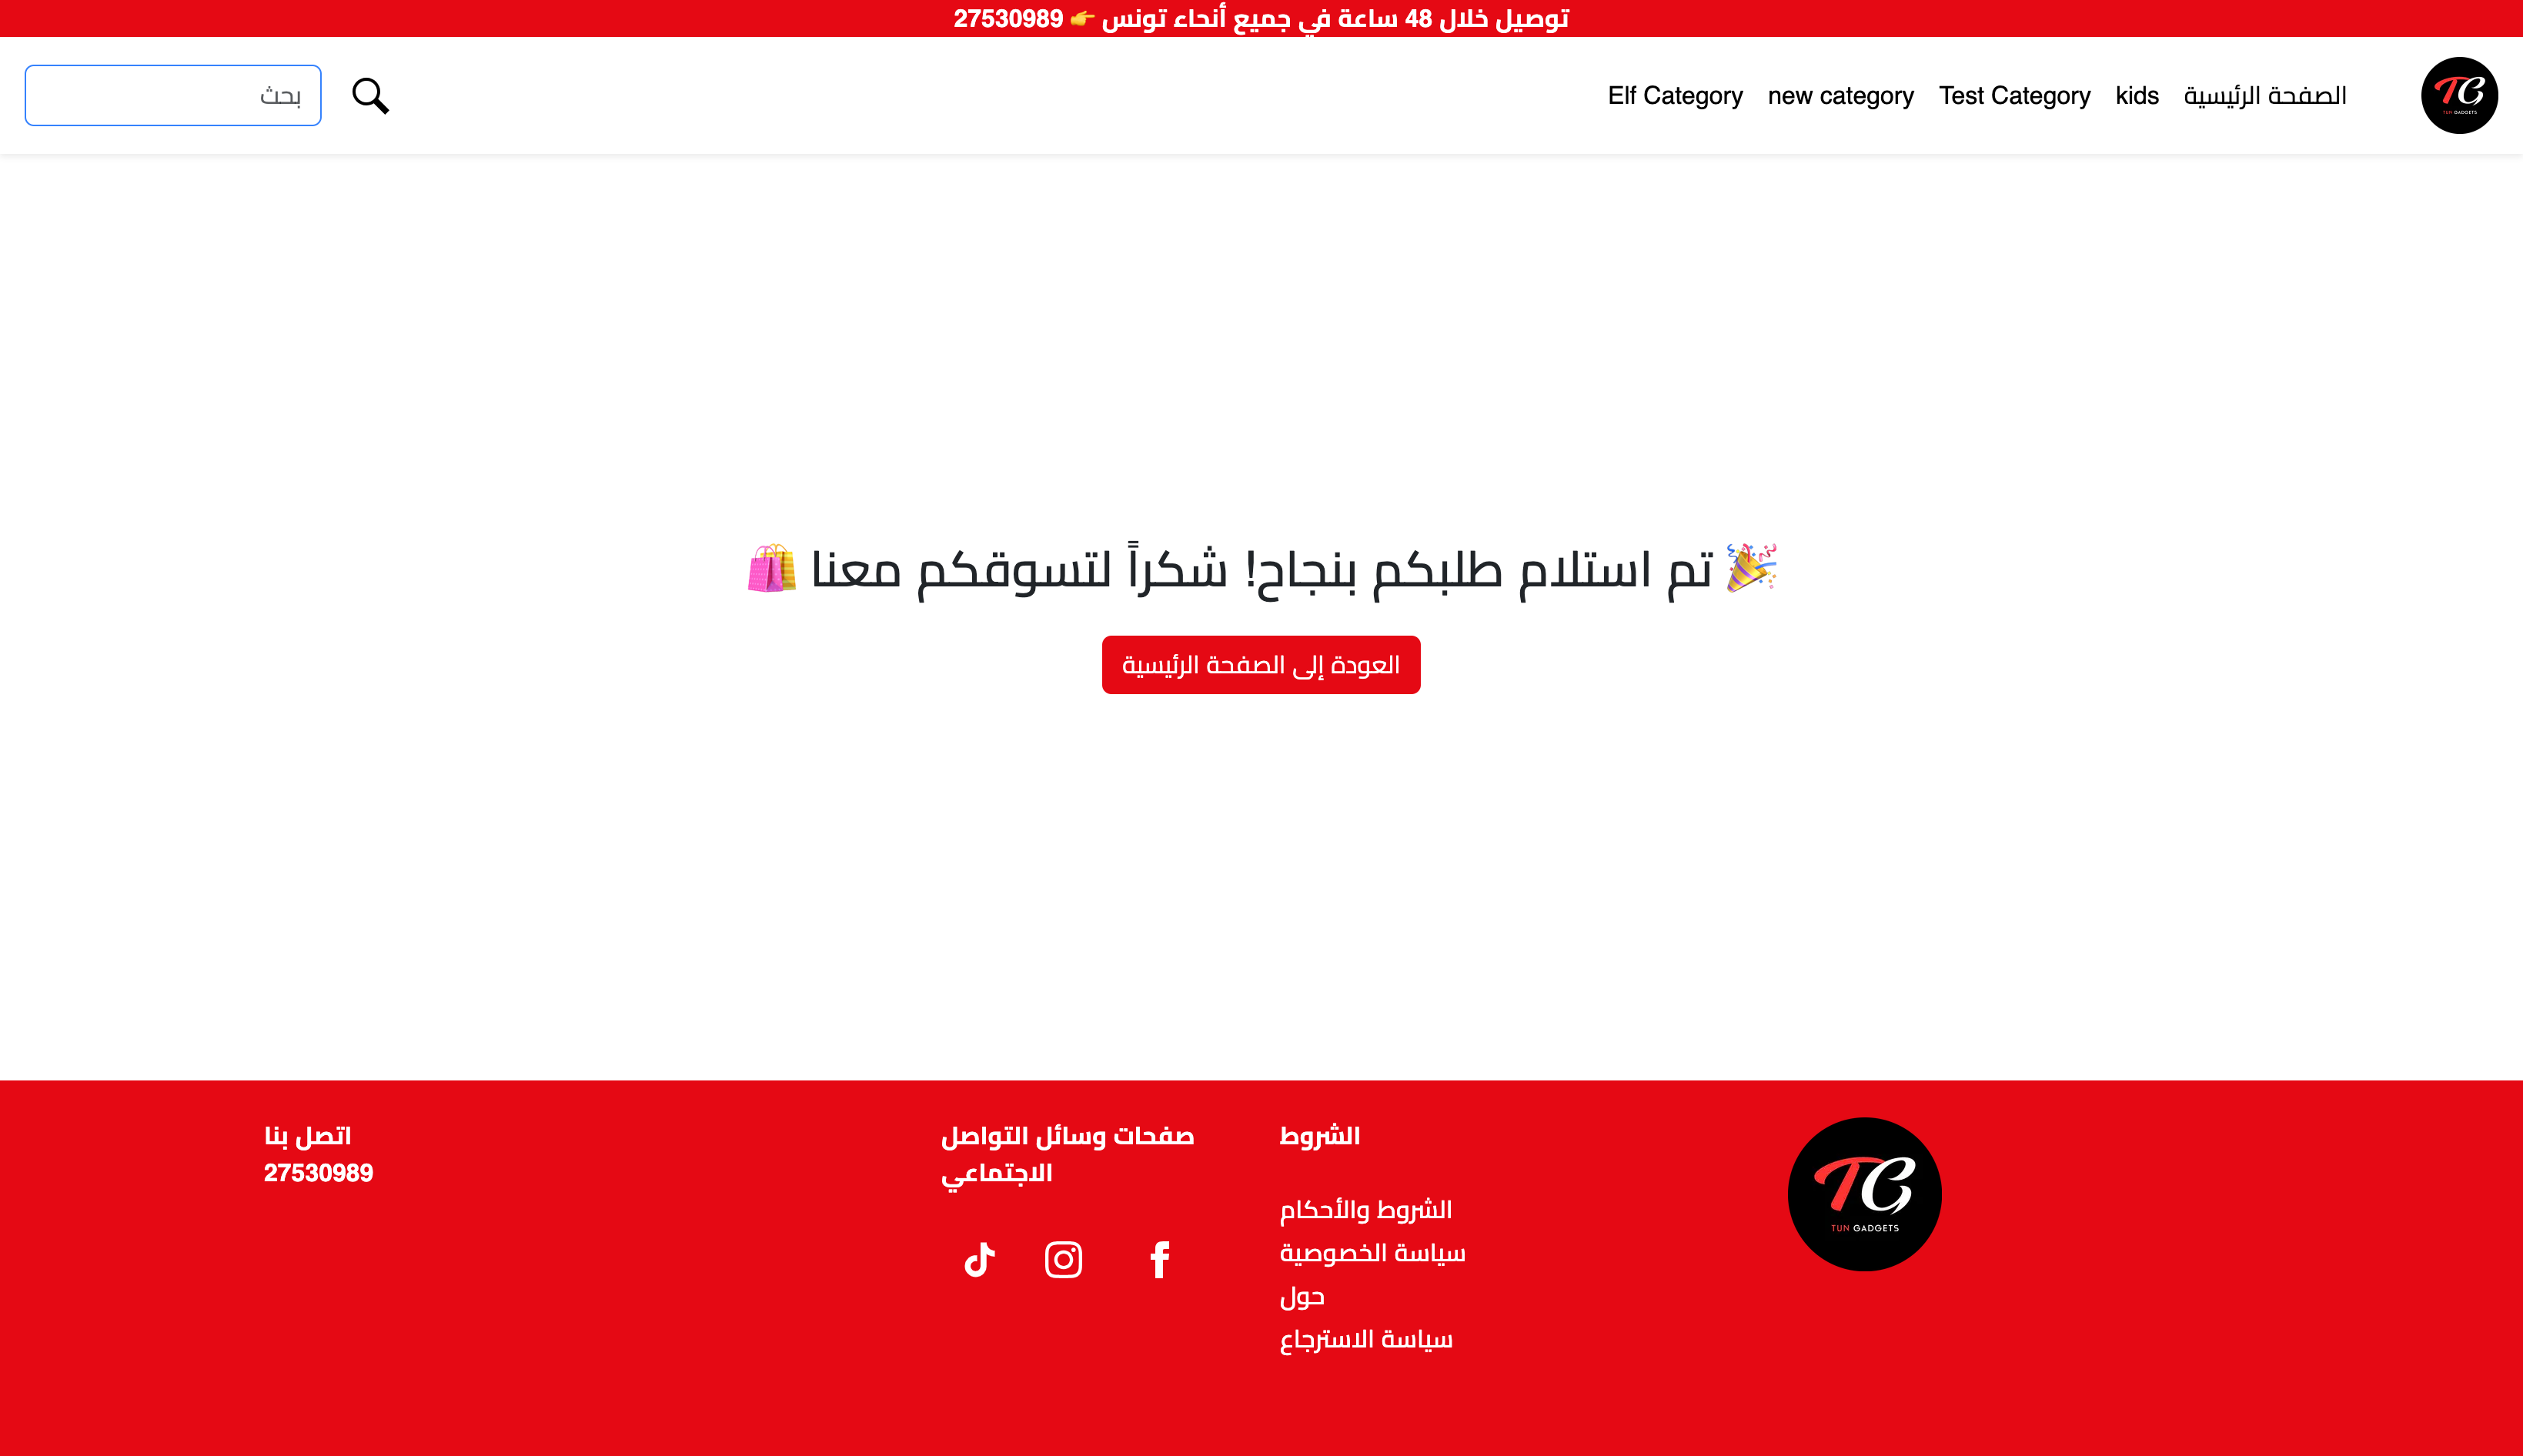
\includegraphics[width=0.8\textwidth]{images/thankYouPage.png}
        \caption{Thank You Page}
        \label{fig:thank_you_page}
    \end{figure}
    \begin{figure}[H]
        \centering
        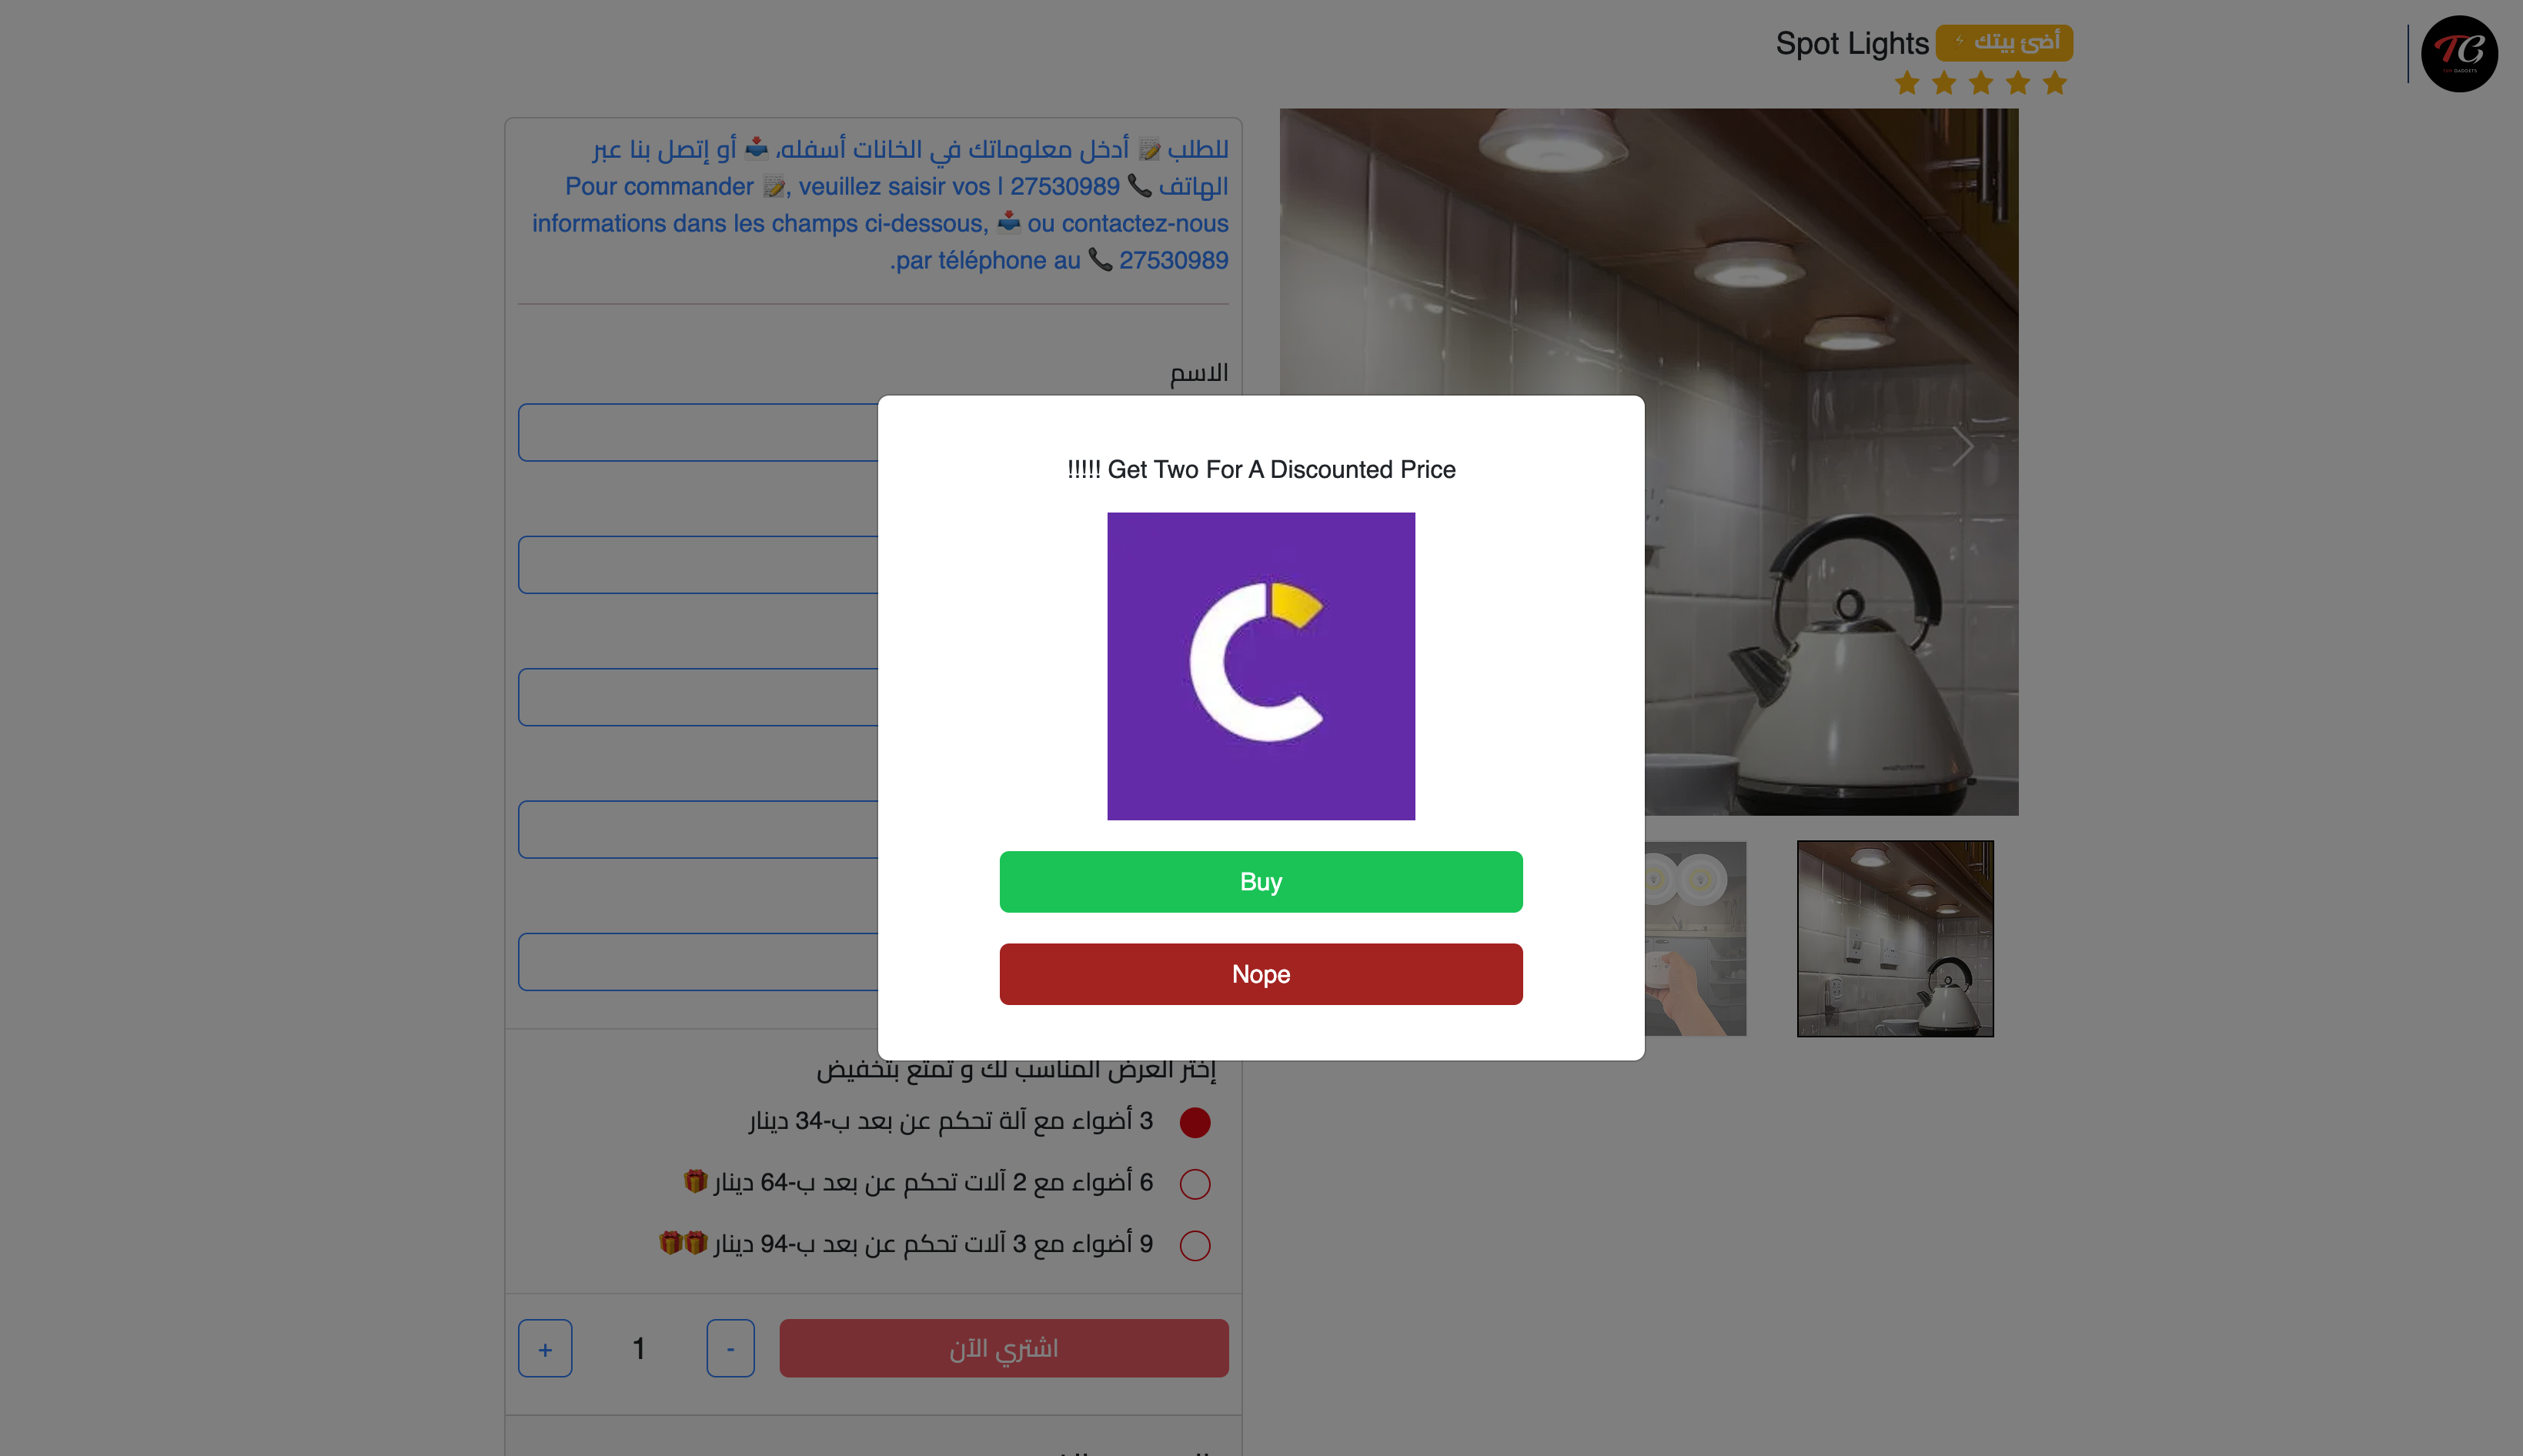
\includegraphics[width=0.8\textwidth]{images/upsell.png}
        \caption{Upsell Popup}
        \label{fig:upsell}
    \end{figure}
\end{itemize}

\subsubsection{Summary}

In this sprint, we successfully recreated the simple template for the shop visiting process. We designed and implemented the frontend components, sequence diagram, and user journey. We also created the various needed pages.

\section{Sprint 2 - Implementing the Upsell/Cross-sell Feature}

\subsection{Sprint Backlog}

In this section, we present the Sprint Backlog, detailing the tasks planned for developing the upsell/cross-sell feature. It is a concise list of user stories and specific actions that will guide us through the sprint.

\setlength{\LTleft}{0pt}
\begin{longtable}{|c|c|c|c|}
\hline
\textbf{Sprint} & \textbf{User Story} & \textbf{Task} & \textbf{ID} \\
\hline
2 & 2.1 & Backend: Implement Read API endpoints for upsells/cross-sells & 2.0.1 \\
\hline
2 & 2.2 & Frontend: Design upsell/cross-sell management UI for Read operations & 2.0.2 \\
\hline
2 & 2.3 & Backend: Implement API endpoints for searching upsells/cross-sells by name. & 2.0.3 \\
\hline
2 & 2.4 & Implement upsell/cross-sell search functionality by name. & 2.0.4 \\
\hline
2 & 2.5 & Backend: Implement API endpoints for editing upsells/cross-sells & 2.0.5 \\
\hline
2 & 2.6 & Frontend: Design upsell/cross-sell management UI for Edit operations & 2.0.6 \\
\hline
2 & 2.7 & Backend: Implement API endpoints for deleting upsells/cross-sells & 2.0.7 \\
\hline
2 & 2.8 & Frontend: Design upsell/cross-sell management UI for Delete operations & 2.0.8 \\
\hline
2 & 2.9 & Frontend: Design upsell/cross-sell management UI for Preview operations & 2.0.9 \\
\hline
\caption{Sprint 2 - Implementing the Upsell/Cross-sell Feature}
\label{tab:sprint2_backlog}
\end{longtable}

\subsection{Design \& Implementation}

In this section, we will explore the design and implementation of the upsell/cross-sell feature. We will begin by examining the backend design and implementation, followed by an analysis of the frontend design.

\subsubsection{Database Schema}

The database schema for the upsell/cross-sell feature is shown in Figure \ref{fig:db_schema_sprint2}. It consists of the following tables:

\begin{figure}[H]
    \centering
    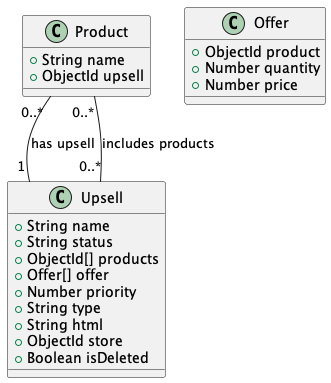
\includegraphics[width=0.5\textwidth]{images/sprintTwoClass.png}
    \caption{Database Schema for Sprint 2}
    \label{fig:db_schema_sprint2}
\end{figure}

The class diagram illustrates the relationships between two main classes: \texttt{Upsell} and \texttt{Product}.

\begin{itemize}
    \item \textbf{Upsell Class:} Represents an upsell with attributes such as an ID (\texttt{\_id}), status, offer, priority, type, HTML, store, and isDeleted. The \texttt{Offer} is a composite object with different attributes like product, quantity, and price.
    
    \item \textbf{Product Class:} Represents a product with attributes like an ID (\texttt{\_id}), name, description, price, and a reference to the \texttt{Upsell}.
    
    \item \textbf{Offer Class:} Contains attributes for the product, quantity, and price.
    
    \item \textbf{Relationships:}
    \begin{itemize}
        \item Each \texttt{Upsell} can include multiple \texttt{Products} through a one-to-many relationship.
        \item Conversely, each \texttt{Product} can have an associated \texttt{Upsell}, maintaining the one-to-one relationship.
    \end{itemize}
\end{itemize}

\subsubsection{Sequence Diagram}

\begin{itemize}
    \item \textbf{Search Operation:} The sequence diagram in Figure \ref{fig:sequence_diagram_sprint2_search} illustrates the interactions between the different components of the search operation. The sequence of events is as follows:
    \begin{figure}[H]
        \centering
        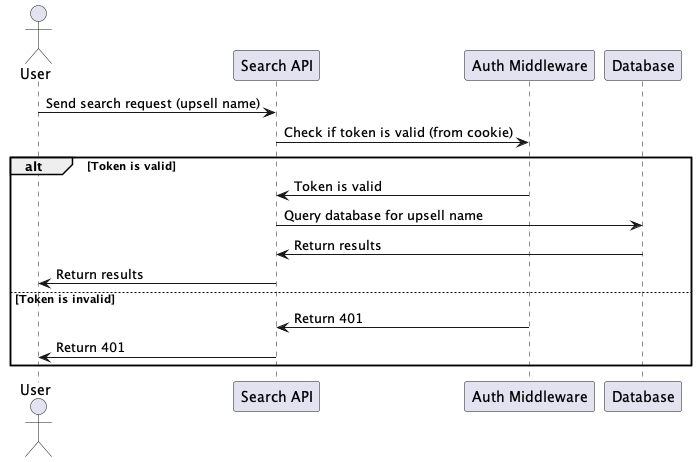
\includegraphics[width=0.8\textwidth]{images/sprintTwoSearchSequence.png}
        \caption{Sequence Diagram for Sprint 2 - Search Operation}
        \label{fig:sequence_diagram_sprint2_search}
    \end{figure}

    \item \textbf{Create Operation:} The sequence diagram in Figure \ref{fig:sequence_diagram_sprint2_create} illustrates the interactions between the different components of the create operation. The sequence of events is as follows:
    \begin{figure}[H]
        \centering
        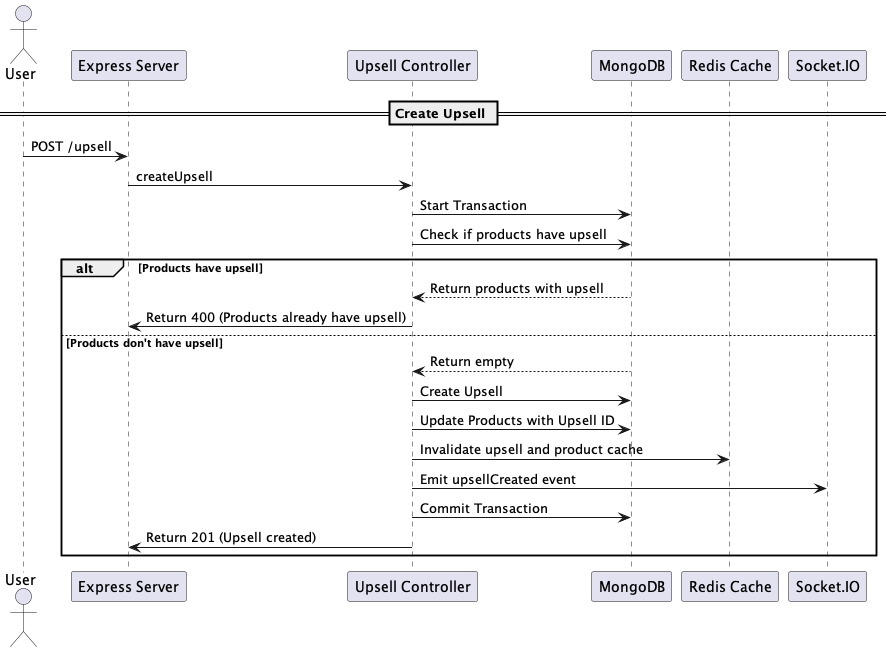
\includegraphics[width=0.8\textwidth]{images/sprintTwoCreateSequence.png}
        \caption{Sequence Diagram for Sprint 2 - Create Operation}
        \label{fig:sequence_diagram_sprint2_create}
    \end{figure}

    \item \textbf{Read Operation:} The sequence diagram in Figure \ref{fig:sequence_diagram_sprint2_read} illustrates the interactions between the different components of the read all operation. The sequence of events is as follows:
    \begin{figure}[H]
        \centering
        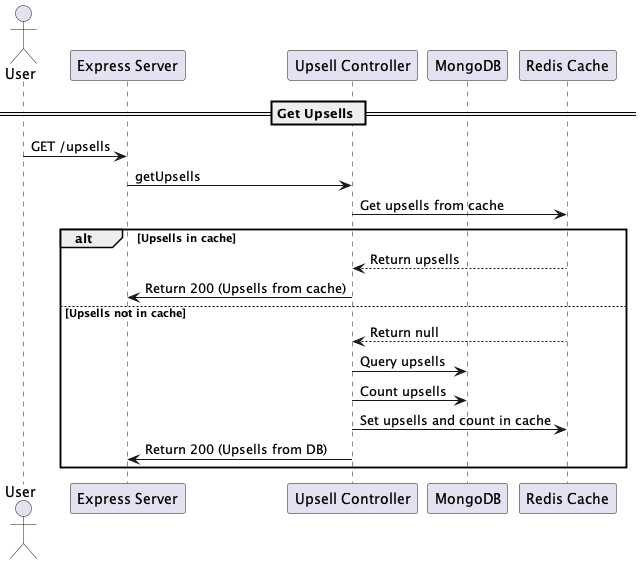
\includegraphics[width=0.8\textwidth]{images/sprintTwoReadAllSequence.png}
        \caption{Sequence Diagram for Sprint 2 - Read Operation}
        \label{fig:sequence_diagram_sprint2_read}
    \end{figure}

    \item \textbf{Update Operation:} The sequence diagram in Figure \ref{fig:sequence_diagram_sprint2_update} illustrates the interactions between the different components of the update operation. The sequence of events is as follows:
    \begin{figure}[H]
        \centering
        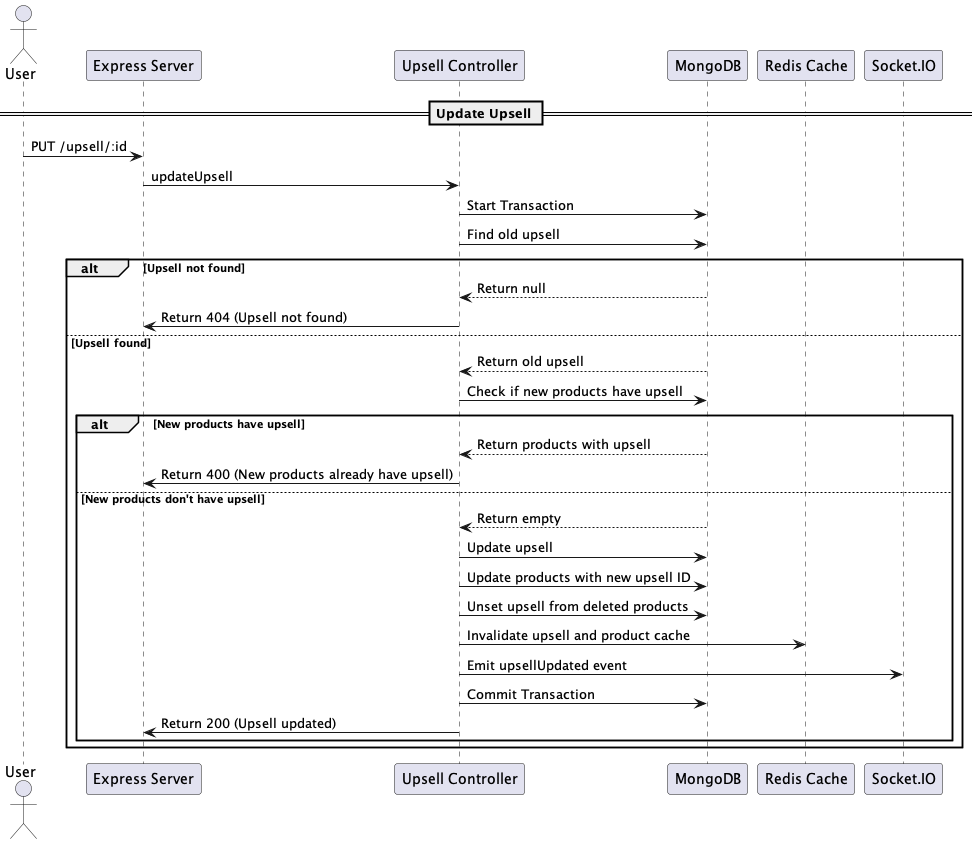
\includegraphics[width=0.8\textwidth]{images/sprintTwoUpdateSequence.png}
        \caption{Sequence Diagram for Sprint 2 - Update Operation}
        \label{fig:sequence_diagram_sprint2_update}
    \end{figure}

    \item \textbf{Delete Operation:} The sequence diagram in Figure \ref{fig:sequence_diagram_sprint2_delete} illustrates the interactions between the different components of the delete operation. The sequence of events is as follows:
    \begin{figure}[H]
        \centering
        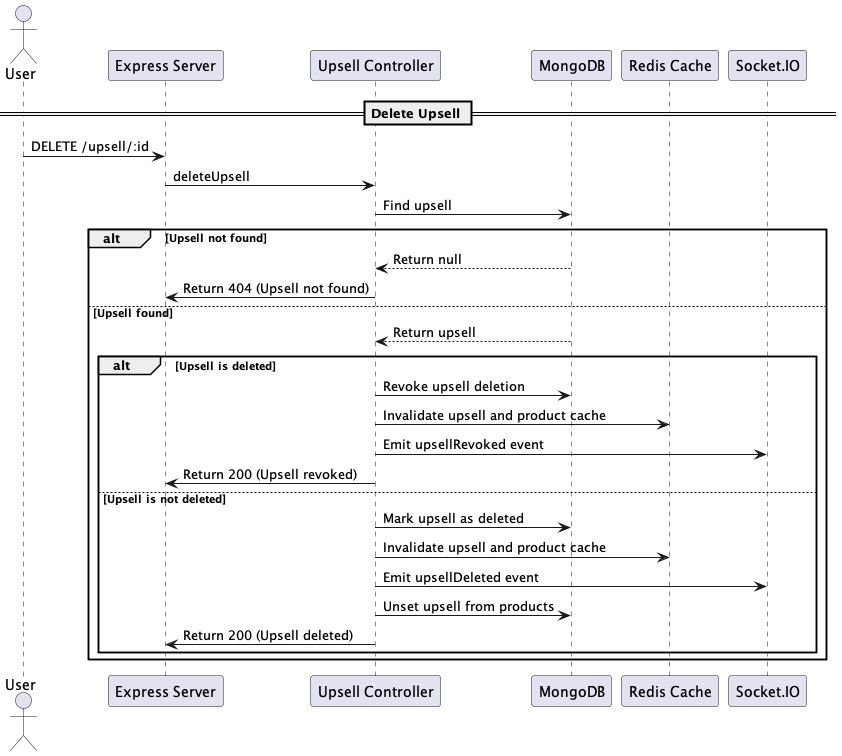
\includegraphics[width=0.8\textwidth]{images/sprintTwoDeleteSequence.png}
        \caption{Sequence Diagram for Sprint 2 - Delete Operation}
        \label{fig:sequence_diagram_sprint2_delete}
    \end{figure}

    \item \textbf{Read One Operation:} The sequence diagram in Figure \ref{fig:sequence_diagram_sprint2_read_one} illustrates the interactions between the different components of the read one operation. The sequence of events is as follows:
    \begin{figure}[H]
        \centering
        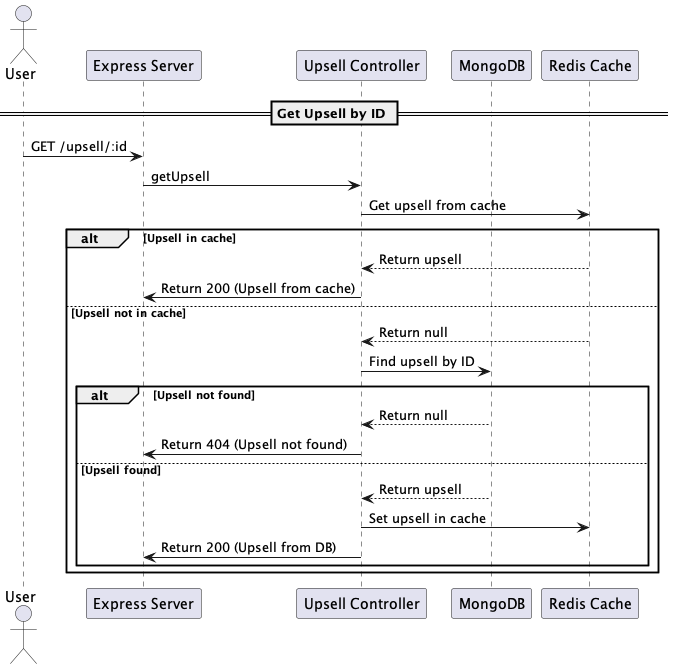
\includegraphics[width=0.8\textwidth]{images/sprintTwoReadOneSequence.png}
        \caption{Sequence Diagram for Sprint 2 - Read One Operation}
        \label{fig:sequence_diagram_sprint2_read_one}
    \end{figure}
\end{itemize}

\subsubsection{Caching Layer}

The caching layer is an essential component of the upsell/cross-sell feature. It helps improve the performance of the application by reducing the number of database queries. The caching layer stores the results of database queries in memory, allowing the application to retrieve data quickly without querying the database each time. The caching layer is implemented using Redis, an open-source, in-memory data structure store.

\begin{figure}[H]
    \centering
    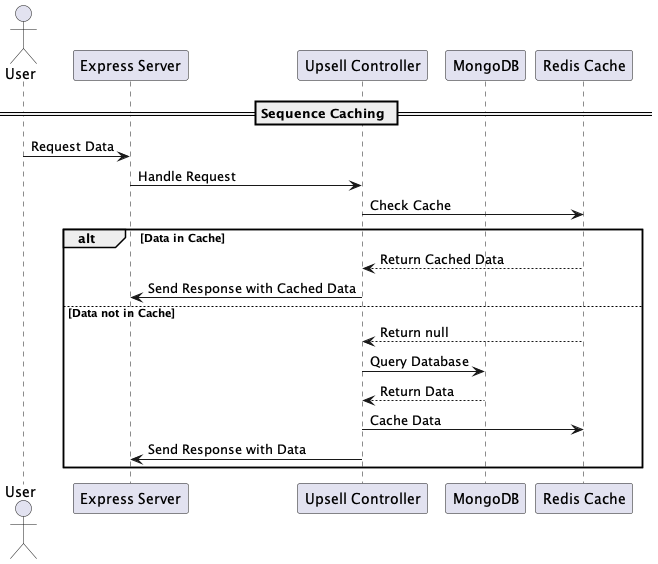
\includegraphics[width=0.8\textwidth]{images/sprintTwoCacheSequence.png}
    \caption{Sequence Diagram for Sprint 2 - Caching Layer}
    \label{fig:sequence_diagram_sprint2_cache}
\end{figure}

Benefits of using a caching layer include:

\begin{itemize}
    \item \textbf{Improved Performance:} By storing data in memory, the application can retrieve it quickly without querying the database each time.
    \item \textbf{Reduced Database Load:} The caching layer reduces the number of database queries, which helps reduce the load on the database server.
    \item \textbf{Scalability:} The caching layer can be scaled horizontally by adding more cache servers to handle increased load.
\end{itemize}

\newpage

And the following is a code snippet of the caching layer implementation:

\begin{lstlisting}[language=Python, caption=Redis Caching Layer Implementation, label=lst:redis_caching_layer, frame=single, framerule=0.5pt]
let data = await redisClient.get(key);

if (data) {
    console.log('Data fetched from Redis');
    return JSON.parse(data);
}
// Data not found in Redis, query MongoDB
const collection = db.collection('mycollection');
data = await collection.findOne({ key });
if (data) {
    console.log('Data fetched from MongoDB');
    redisClient.setex(key, 3600, JSON.stringify(data));
    return data;
}
\end{lstlisting}

\subsubsection{User Journey}

The user journey for the upsell/cross-sell creation feature is as follows:

\begin{figure}[H]
    \centering
    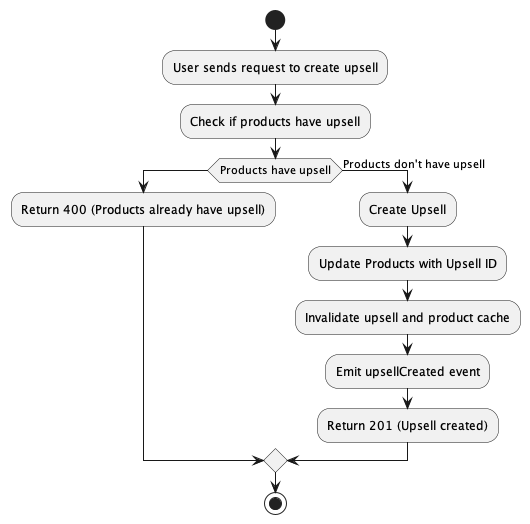
\includegraphics[width=0.8\textwidth]{images/sprintTwoActivity.png}
    \caption{User Journey for Sprint 2}
    \label{fig:user_journey_sprint2}
\end{figure}

\subsubsection{Screenshots - UI Design}

\begin{itemize}
    \item \textbf{Table View Dashboard :} The table view dashboard displays a list of upsells/cross-sells in a tabular format. Figure \ref{fig:table_view_dashboard} shows the table view dashboard.
    \begin{figure}[H]
        \centering
        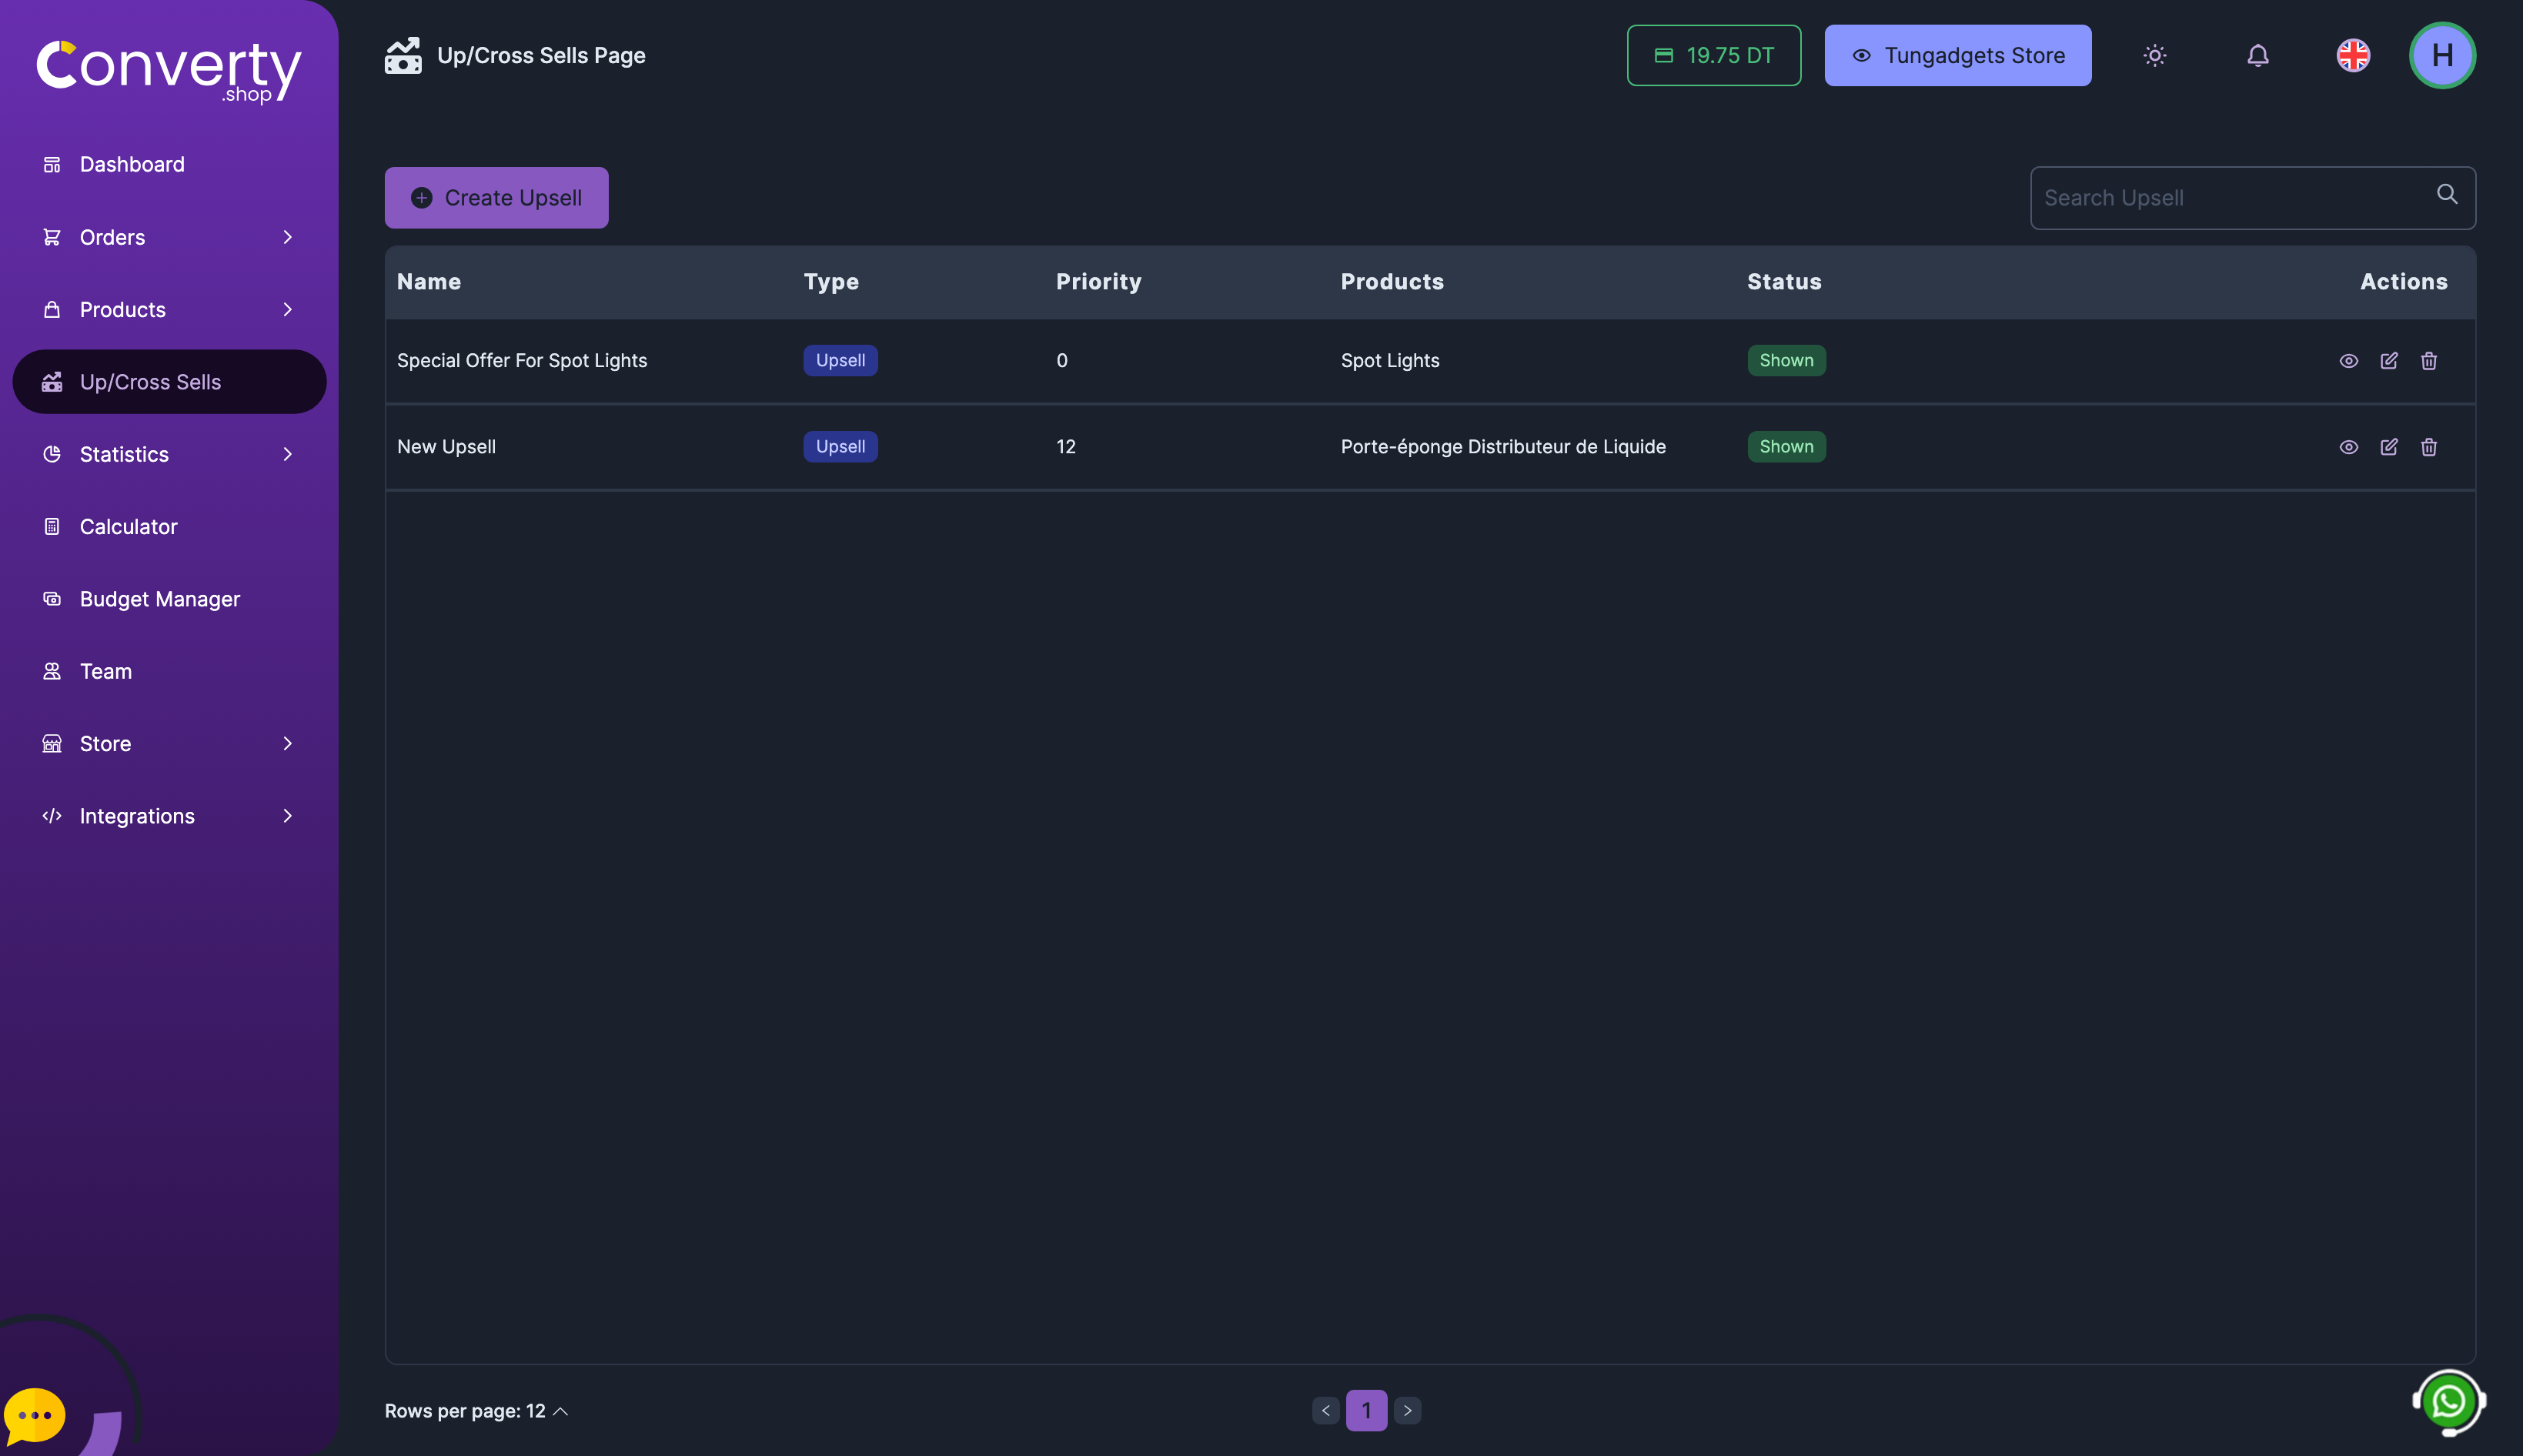
\includegraphics[width=0.8\textwidth]{images/tableViewDashboard.png}
        \caption{Table View Dashboard}
        \label{fig:table_view_dashboard}
    \end{figure}
    \item \textbf{Upsell/Cross-sell Preview:} The upsell/cross-sell preview displays a preview of the upsell/cross-sell. Figure \ref{fig:upsell_preview} shows the upsell/cross-sell preview.
    \begin{figure}[H]
        \centering
        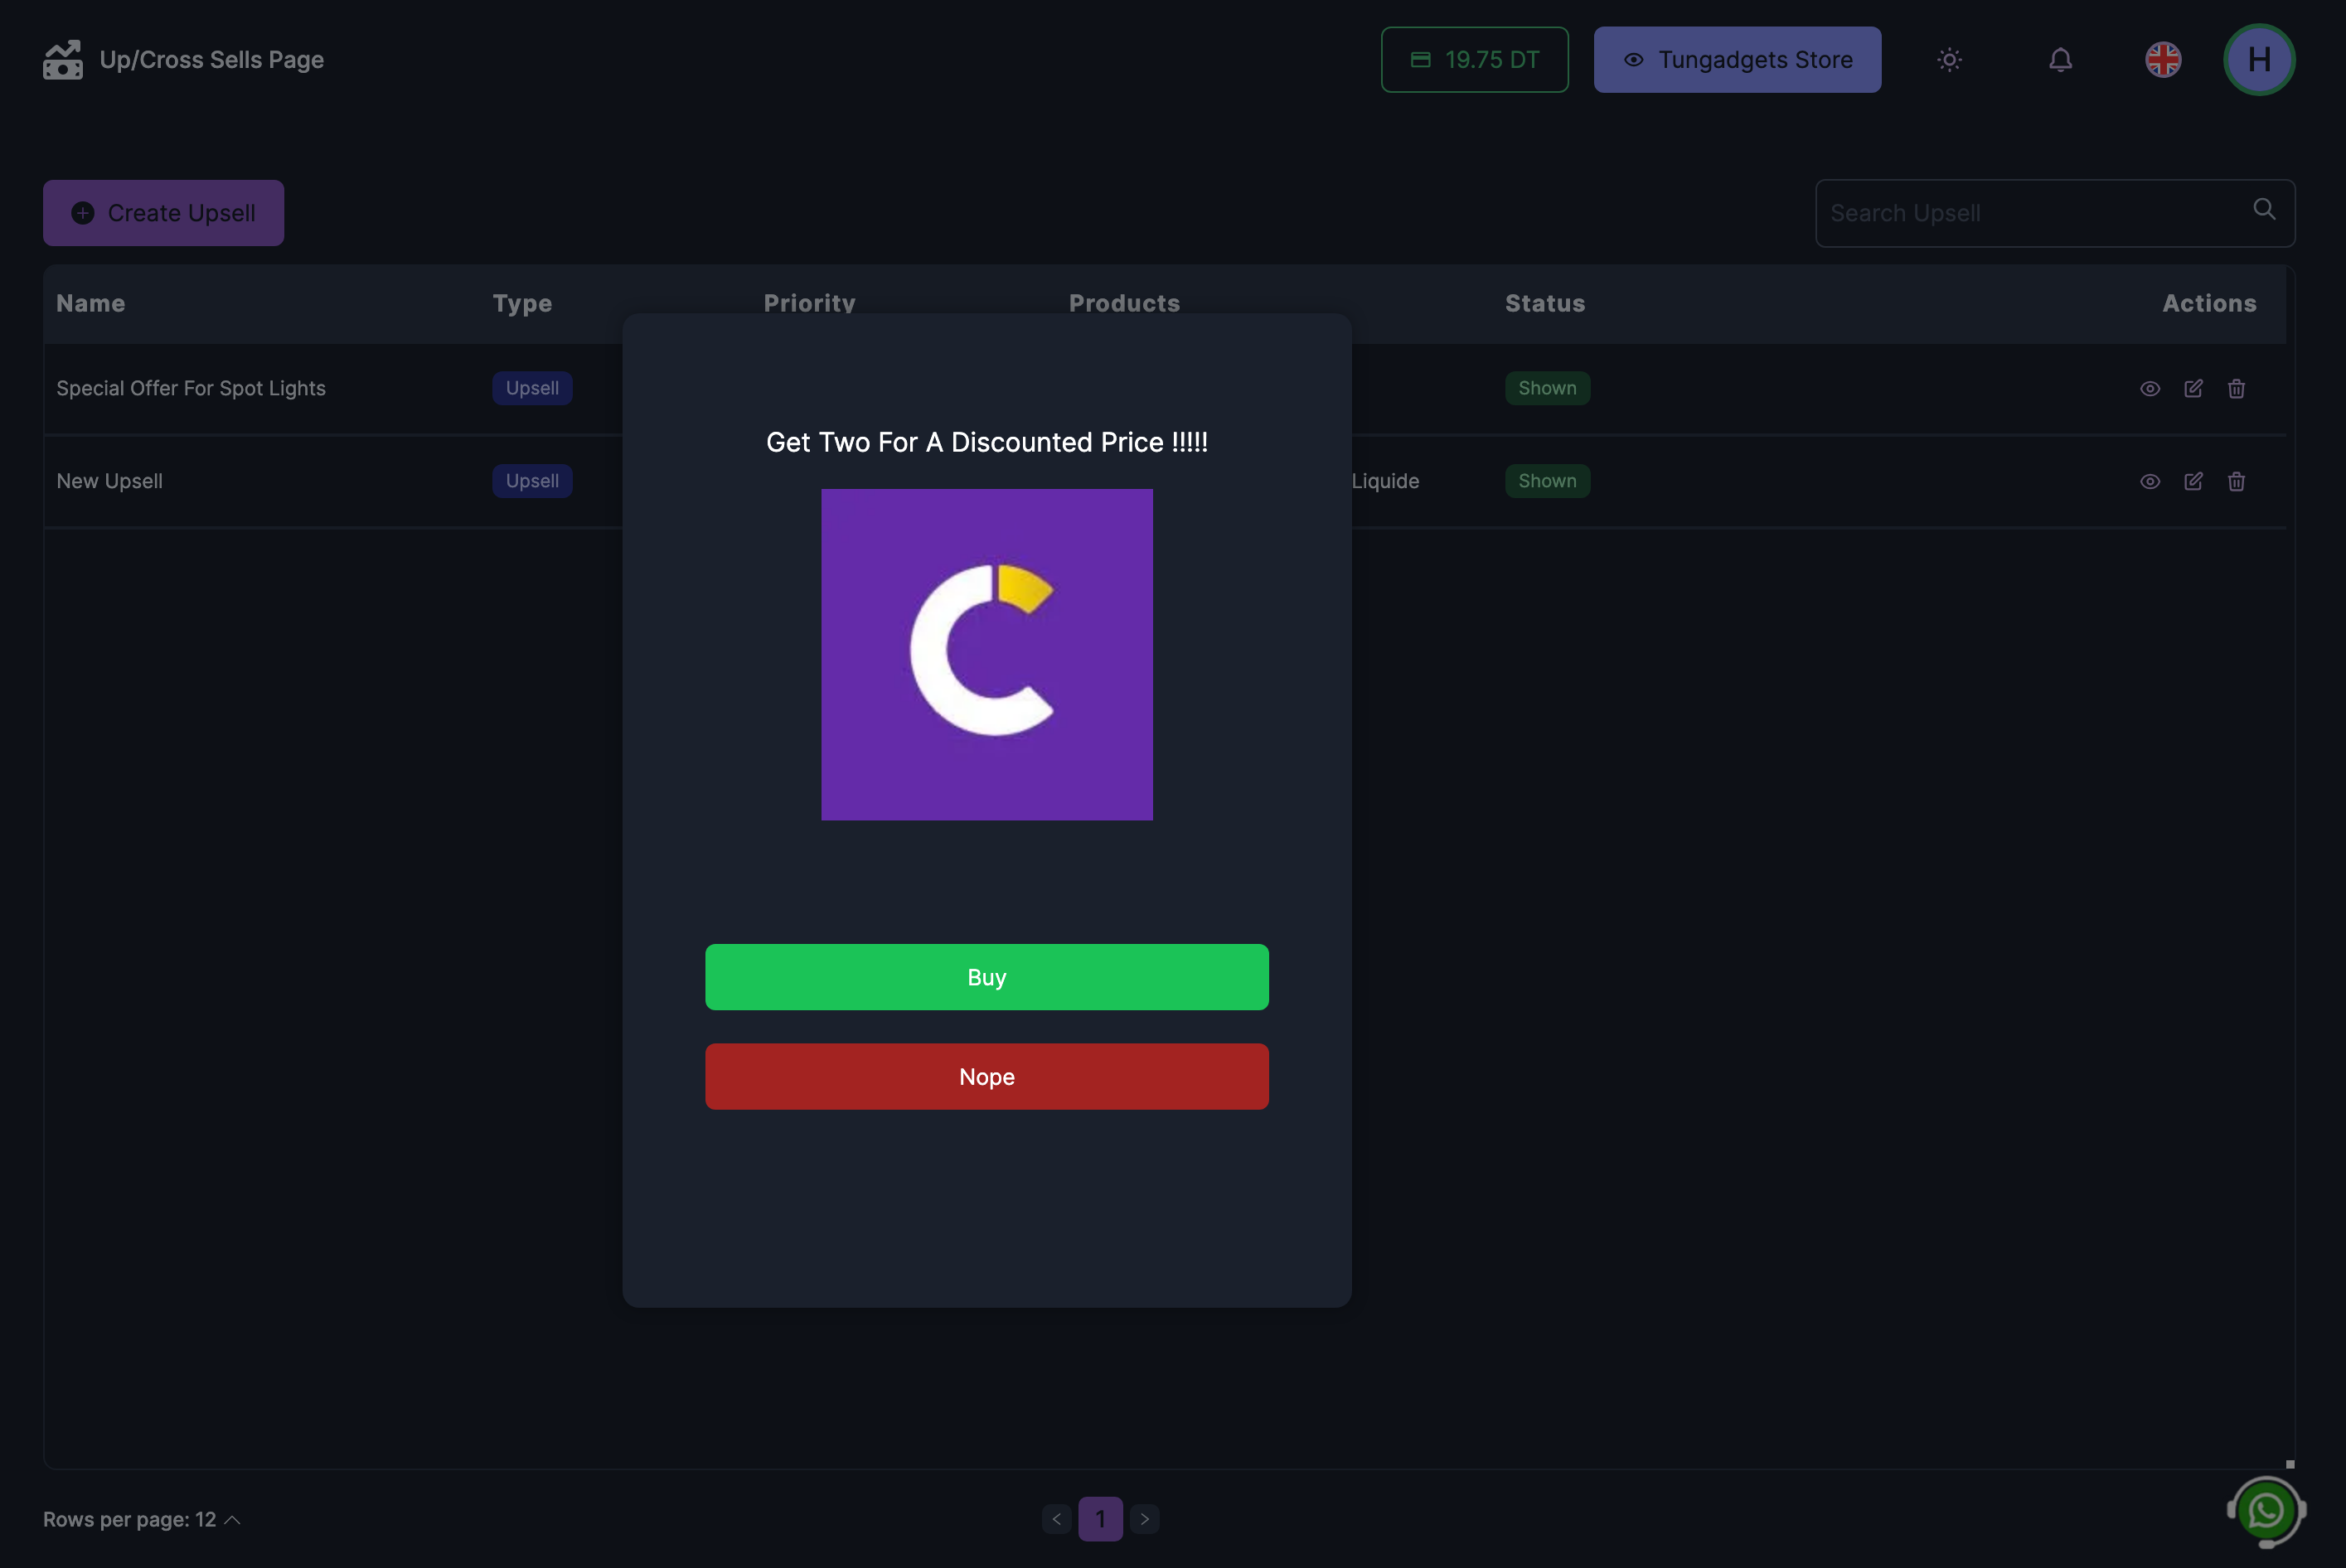
\includegraphics[width=0.8\textwidth]{images/upsellPreview.png}
        \caption{Upsell/Cross-sell Preview}
        \label{fig:upsell_preview}
    \end{figure}
    \item \textbf{Edit/Add Upsell/Cross-sell:} The edit/add upsell/cross-sell page allows users to create or edit an upsell/cross-sell. Figures \ref{fig:edit_upsell_one} and \ref{fig:edit_upsell_two} shows the edit/add upsell/cross-sell page.
    \begin{figure}[H]
        \centering
        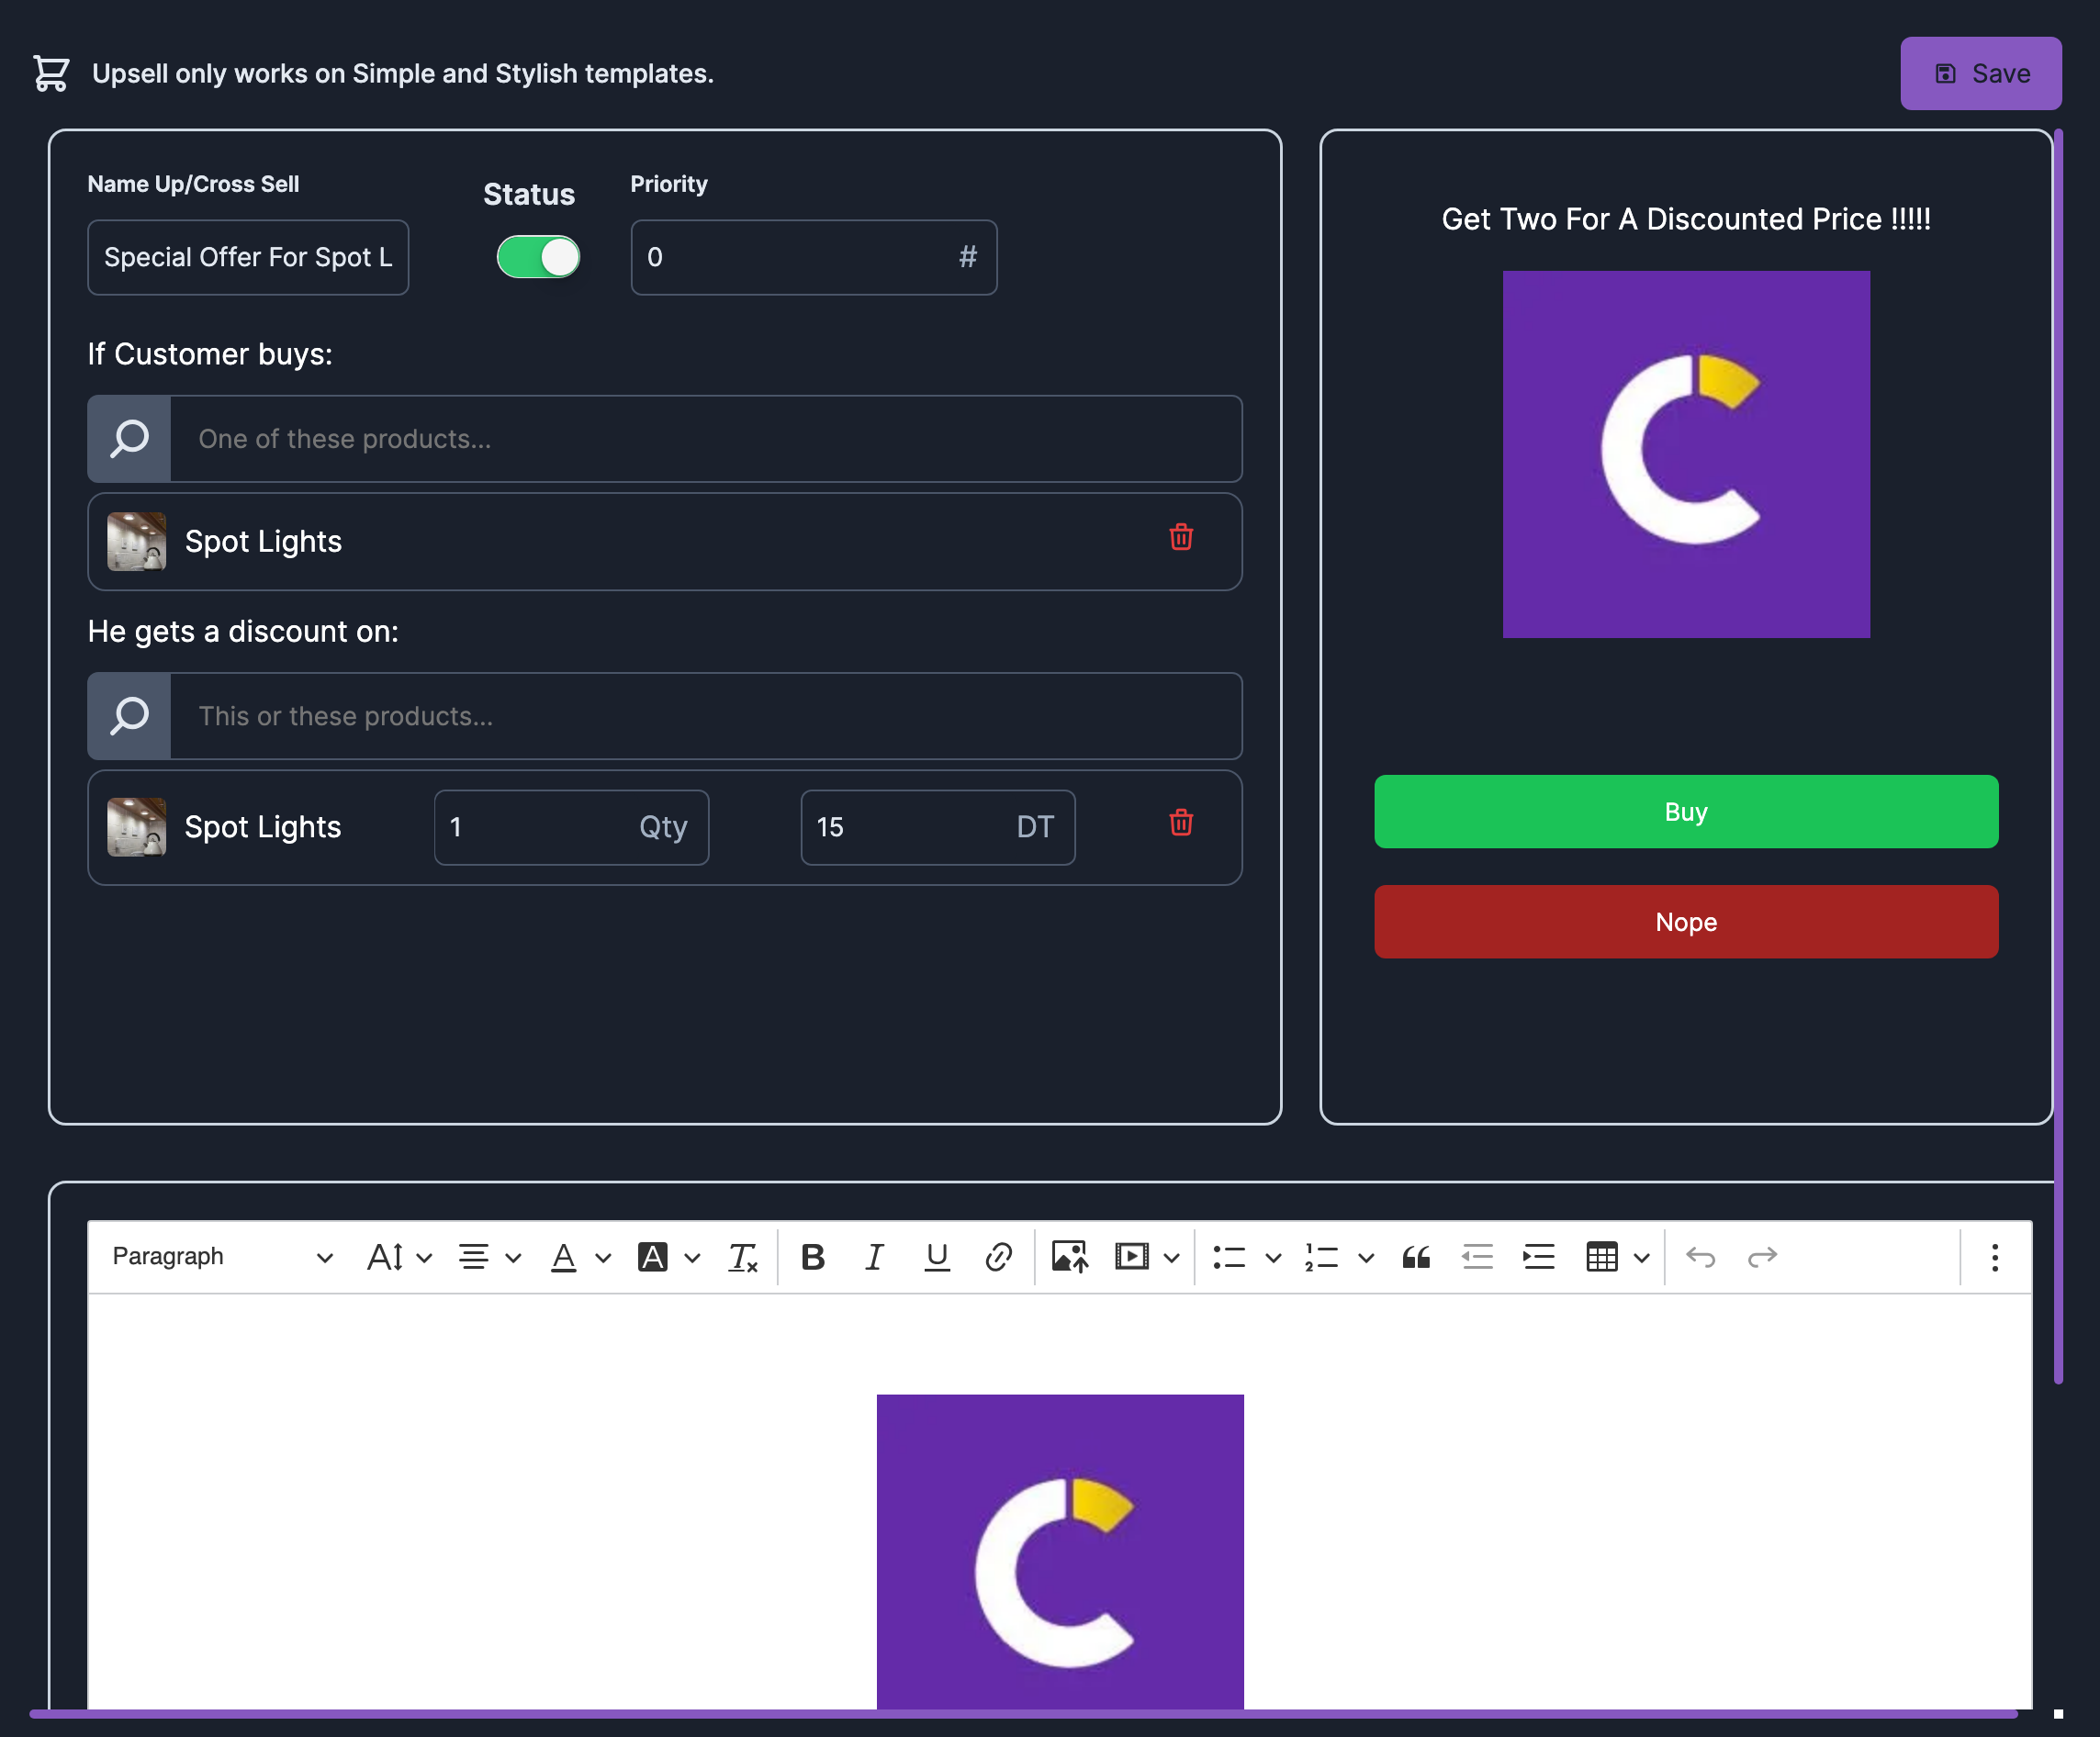
\includegraphics[width=0.8\textwidth]{images/editUpsell1.png}
        \caption{Edit/Add Upsell/Cross-sell 1}
        \label{fig:edit_upsell_one}
    \end{figure}
    \begin{figure}[H]
        \centering
        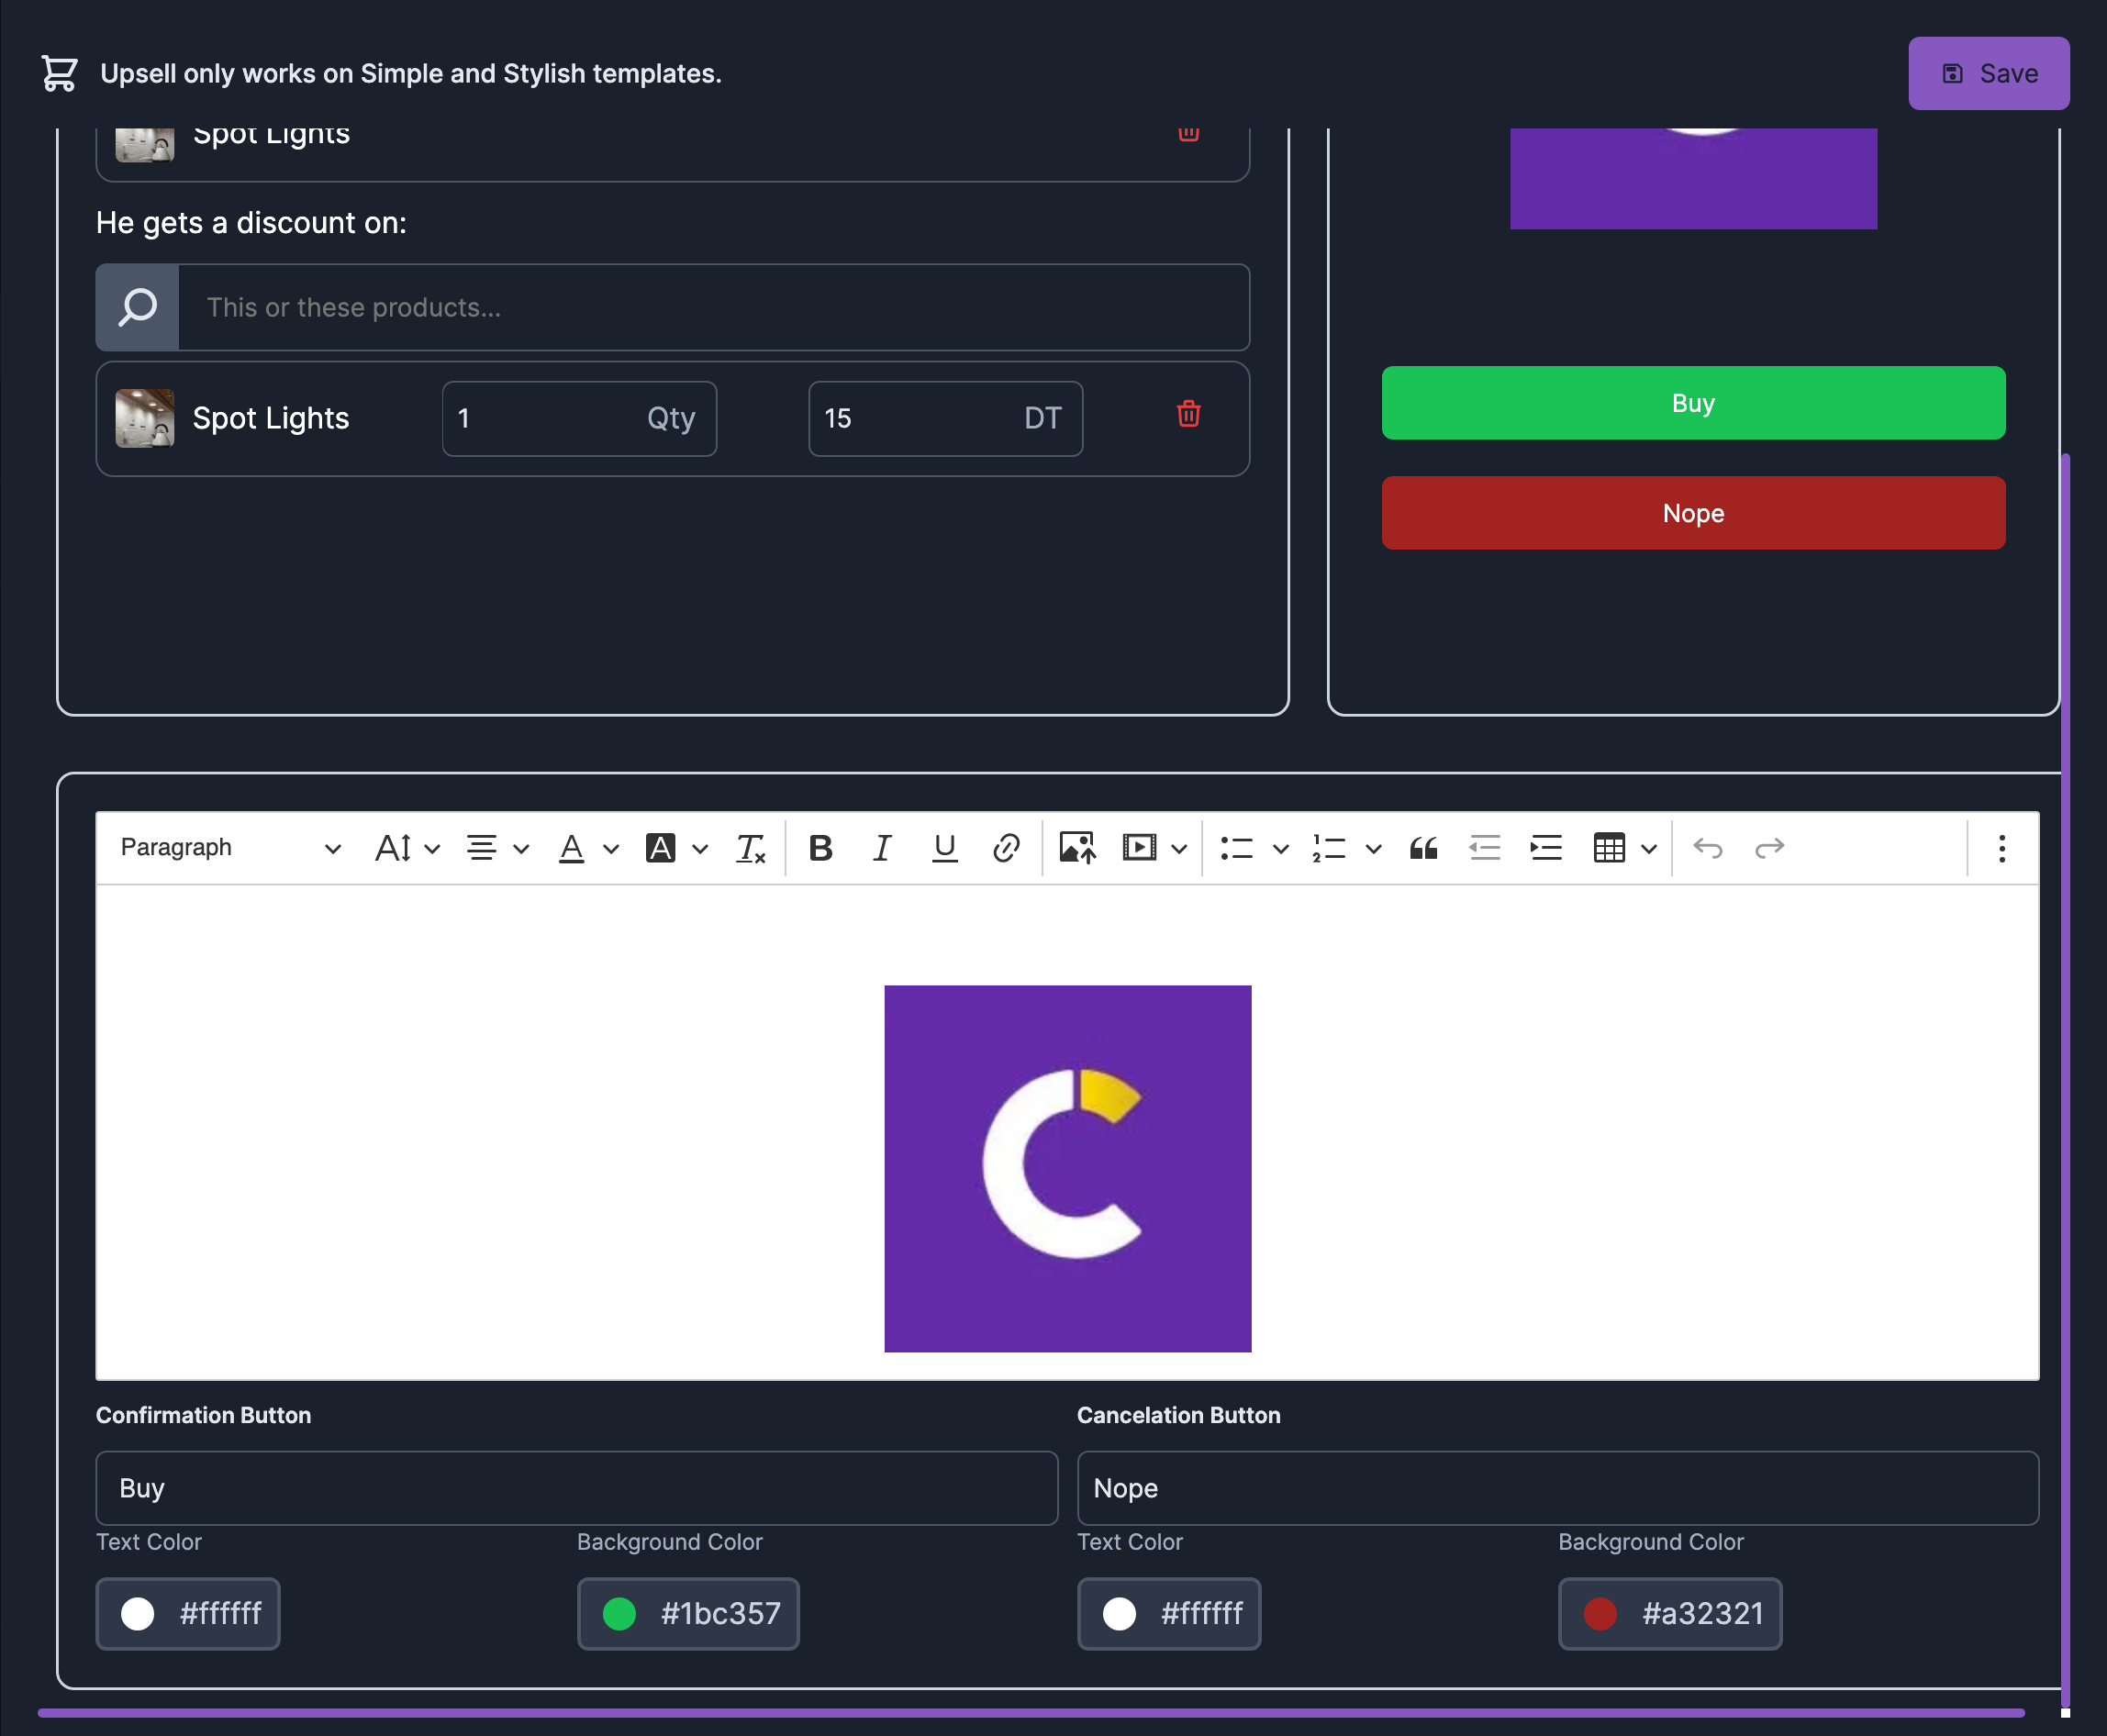
\includegraphics[width=0.8\textwidth]{images/editUpsell2.png}
        \caption{Edit/Add Upsell/Cross-sell 2}
        \label{fig:edit_upsell_two}
    \end{figure}
\end{itemize}

\subsubsection{Summary}

In this sprint, we successfully implemented the upsell/cross-sell feature. We designed and implemented the frontend and backend components, sequence diagrams, and user journey. We also created the various needed pages.

\section{Conclusion}

In this chapter, we discussed the two web-related sprints. We provided a detailed explanation of the conception part, including a class diagram and a sequence diagram. Additionally, we presented the sprint backlog and included relevant screenshots of these sprints. Furthermore, we showcased some code snippets to illustrate the implementation process.